% \documentclass[10pt,conference]{IEEEtran}

\documentclass[acmtosem, screen ,review]{acmart}

\usepackage[utf8]{inputenc}

\AtBeginDocument{%
  \providecommand\BibTeX{{%
    Bib\TeX}}}

    
%\IEEEoverridecommandlockouts

\settopmatter{printacmref=false}

\setcopyright{none}
\settopmatter{printfolios=true}

\usepackage{pifont}
\usepackage{xcolor}
\definecolor{codepurple}{rgb}{0.58,0,0.82}
\definecolor{framecolor}{RGB}{0,0,0}
\definecolor{backcolor}{RGB}{245,245,245}
\definecolor{titlecolor}{RGB}{70,70,70}
\definecolor{bleu}{rgb}{0.0,0.0,1.0}
\definecolor{codegray}{rgb}{0.5,0.5,0.5}
\definecolor{darkblue}{rgb}{0.5,0.5,0.5}
\definecolor{formalshade}{rgb}{.9,.9,.9}
\definecolor{codegreen}{rgb}{0,0.5,0}

\usepackage{graphicx}
\graphicspath{{figures/}{figures/Result_figures/}{Birdirectional-ICSE/figures/}{Birdirectional-ICSE/figures/Result_figures/}}
\usepackage{booktabs}
\usepackage{tabularx}
\usepackage{subcaption}
\usepackage{fontawesome5}
\usepackage{mdframed}
\usepackage{amsmath}
\usepackage{adjustbox}
\usepackage{amsthm}
\newtheorem{definition}{Definition}
\usepackage{enumitem}
\let\Bbbk\relax
\usepackage{amssymb}
\usepackage{amsmath}
\usepackage{ifthen}
\usepackage{textcomp}
\usepackage{pgfplots}
\pgfplotsset{compat=1.18}
\usepgfplotslibrary{statistics}
\usepackage{tcolorbox}
\usepackage{siunitx}
\usepackage{algorithm}
\usepackage{algorithmic}
\usepackage{framed}
\usepackage{changepage}
\usepackage{listings}
\usepackage{balance}
\usepackage{tikz}
\usetikzlibrary{arrows.meta,positioning,shapes.geometric,shadows}
\usepackage{placeins}
%\usepackage{cite}
\usepackage{hyperref}
\usepackage[nameinlink]{cleveref}
\usepackage{makecell}
\renewcommand\theadalign{lc}

\newcommand{\cmark}{\ding{51}}
\newcommand{\xmark}{\ding{55}}
\newcommand{\wcircle}[1]{\ding{\numexpr171 + #1}}
\newcommand{\bcircle}[1]{\ding{\numexpr181 + #1}}

\mdfdefinestyle{niceframe}{
    linewidth=1pt,
    linecolor=framecolor,
    backgroundcolor=gray!25,
    roundcorner=5pt,
    innertopmargin=\baselineskip,
    frametitlefont=\bfseries\sffamily\color{titlecolor},
    frametitlealignment=\raggedright,
    frametitlebackgroundcolor=gray!25,
    shadow=true,
    shadowsize=3pt,
    shadowcolor=black!20,
}

\newenvironment{formal}{%
  \def\FrameCommand{%
    \hspace{0pt}%
    {\color{darkblue}\vrule width 2pt}%
    {\color{formalshade}\vrule width 0pt}%
    \colorbox{formalshade}%
  }%
  \MakeFramed{\advance\hsize-\width\FrameRestore}%
  \noindent\hspace{-4.55pt}%
  \begin{adjustwidth}{}{8pt}%
  \ding{43} \textbf{Finding.}
}
{%
  \end{adjustwidth}\endMakeFramed%
}

\lstset{%
	basicstyle={\footnotesize\ttfamily},
	numbers=left,numberstyle=\footnotesize,xleftmargin=2em,
	aboveskip=0pt,belowskip=0pt,
	showstringspaces=false,tabsize=2,breaklines=true,
    commentstyle=\color{codegreen},
    keywordstyle=\color{magenta},
    stringstyle=\color{codepurple},
    numberstyle=\tiny\color{codegray},
    breakatwhitespace=false,
    captionpos=b,
    keepspaces=true,
    numbers=left,
    numbersep=5pt,
    showspaces=false,
    showstringspaces=false,
    showtabs=false
}

\urlstyle{rm}
\def\UrlFont{\rm}

\newboolean{showcomments}
\setboolean{showcomments}{true}
\ifthenelse{\boolean{showcomments}}
 { \newcommand{\mynote}[2]{
      \fbox{\bfseries\sffamily\scriptsize#1}
        {\small$\blacktriangleright$\textsf{\emph{#2}}$\blacktriangleleft$}}}

\newcommand{\finding}[1]{
	\setlength{\fboxrule}{1pt}
	\begin{center}\
		\noindent\fcolorbox{black}{gray!10}{
		\begin{minipage}{.92\linewidth}
			#1
		\end{minipage}
	}
	\end{center}
	\smallskip
}

\newcommand{\se}[1]{\mynote{Serge}{\textcolor{blue}{#1}}}
\newcommand{\js}[1]{\mynote{Jordan}{\textcolor{red}{#1}}}
\newcommand{\tb}[1]{\mynote{Bissyande}{\textcolor{red}{#1}}}
\newcommand{\ak}[1]{\mynote{Kader}{\textcolor{red}{#1}}}

\newcommand{\rqanswer}[2]{%
  \begin{tcolorbox}[leftrule=0.4mm,rightrule=0mm,toprule=0mm,bottomrule=0mm,left=0pt,right=0pt,top=0pt,bottom=0pt]
  \textbf{[RQ-#1] \ding{42}} \textit{#2}
  \end{tcolorbox}
}

%\title{Directional Capability Loss \\in Fine-Tuned Code LLMs}
%\title{LLM Fine-Tuning Induces Directional Forgetting \\in Paired Code Transformations}
%\title{The Inversion Curse in LLM Fine-Tuning \\ for Paired Code Transformations
 %}
% \author{\IEEEauthorblockN{Anonymous Author(s)}
% % \IEEEauthorblockA{Anonymous Institution\\
% % anonymous@anonymous.org}
% }

\begin{document}


\title{
%When Metrics Miss the Mark: Revealing the Fragility of Semantic Similarity Metrics with Trivial Mutations
The Inversion Curse in LLM Fine-Tuning for Paired Code Transformations}


\author{Serge Lionel Nikiema}
\orcid{0009-0001-0066-3694}
\authornote{Corresponding author (lionel.nikiema@uni.lu)}
\affiliation{%
  \institution{University of Luxembourg}
  \city{Luxembourg}
  \country{Luxembourg}
}
\email{}

\author{Jordan SAMHI}
\orcid{0000-0001-6052-6184}
\affiliation{%
  \institution{University of Luxembourg}
  \city{Luxembourg}
  \country{Luxembourg}
}
\email{jordan.samhi@uni.lu}


\author{Micheline Bénédicte Moumoula}
\orcid{0009-0005-1206-2270}
\affiliation{%
  \institution{University of Luxembourg }
  \city{Luxembourg}
  \country{Luxembourg}
}
\email{micheline.moumoula@uni.lu}

\author{Albérick Euraste Djiré}
\orcid{0009-0007-0406-9573}
\affiliation{%
  \institution{University of Luxembourg}
  \city{Luxembourg}
  \country{Luxembourg}
}
\email{euraste.djire@uni.lu}


\author{Abdoul Kader Kaboré}
\orcid{0000-0002-3151-9433}
\affiliation{%
  \institution{University of Luxembourg}
  \city{Luxembourg}
  \country{Luxembourg}
}
\email{abdoulkader.kabore@uni.lu}

\author{Jacques Klein}
\orcid{0000-0003-4052-475X}
\affiliation{%
  \institution{University of Luxembourg}
  \city{Luxembourg}
  \country{Luxembourg}
}
\email{jacques.klein@uni.lu}

\author{Tegawendé F. Bissyandé}
\orcid{0000-0001-7270-9869}
\affiliation{%
  \institution{University of Luxembourg}
  \city{Luxembourg}
  \country{Luxembourg}
}
\email{tegawende.bissyande@uni.lu}

\renewcommand\shortauthors{NIKIEMA et al.}



\begin{abstract}

Many software engineering tasks come in pairs (e.g., translate/back-translate java to/from python). Yet, fine-tuned LLMs are usually evaluated only on the direction they were
trained to generate. We show that this practice can conceal a
software-engineering-relevant failure mode in which forward performance improves
while the corresponding inverse capability degrades. We propose
the Bidirectional Reasoning Framework (BRF), which measures this effect by evaluating a fine-tuned model
on both a transformation and its inverse. Our study covers three paired software
engineering settings: \wcircle{1} obfuscation and deobfuscation, \wcircle{2} translation and back-translation, and \wcircle{3} compilation and decompilation. Obfuscation serves as the
primary controlled testbed, since forward pairs are abundant, reverse
supervision is scarce, and the inverse tasks range from lexical rewriting to
structural and semantic recovery. Across six LLMs, three semantics-preserving
obfuscation types, and four prompting strategies, standard fine-tuning raises
forward accuracy from below 5\% to between 12\% and 81.3\%, depending on transformation complexity, while reverse deobfuscation accuracy falls to 0\% regardless of that variation. The reverse outputs remain executable and semantically valid,
yet they stay near-verbatim copies of the obfuscated input rather than moving
back toward the original readable program. A chain-of-thought probe on lexical
obfuscation finds that a model can state the correct reverse mapping in its
reasoning trace and still emit the forward-style output. Balanced bidirectional
fine-tuning recovers reverse accuracy on lexical and structural tasks, whereas
contrastive fine-tuning recovers it only on identifier renaming, from 0\% to
43\% average across models, without any reverse labels. The two additional settings exhibit the same
direction of effect. Forward-only fine-tuning on Python-to-Java lowers
Java-to-Python test-pass accuracy from 85.4\% to 63.3\%, and forward-only
fine-tuning on C-to-assembly lowers assembly-to-C re-execution accuracy from
16.5\% to 5.5\%. The evidence argues that any code LLM intended for a task with a
meaningful inverse should be evaluated in both directions before deployment.

\end{abstract}

% \begin{IEEEkeywords}
% Inversion Curse, Directional Capability Loss, Bidirectional Reasoning, Fine-Tuning,  LLMs
% \end{IEEEkeywords}

\keywords{Inversion Curse, Directional Capability Loss, Bidirectional Reasoning, Fine-Tuning, LLMs}

\maketitle

\section{Introduction}
\label{sec:introduction}

Many software engineering tasks come in pairs. Obfuscation and
deobfuscation~\cite{yadegari2015generic}, translation and
back-translation~\cite{lachaux2021unsupervised,pan2024lost}, and compilation and
decompilation~\cite{tan2024llm4decompile}each require a model to move between two related representations of the same program. Yet fine-tuning practice evaluates only the direction on which the model was trained. A given LLM can therefore be judged
successful after it improves on the trained transformation, even when it has lost
the inverse capability that developers rely on for inspection, migration,
debugging, and reverse engineering.

This paper asks whether forward fine-tuning preserves the reverse capability of LLMs. We ground the question in three paired settings: \wcircle{1} obfuscation and
deobfuscation, \wcircle{2} translation and back-translation, and \wcircle{3} compilation and
decompilation. Obfuscation provides the primary controlled testbed. Its forward
direction is cheap to supervise with existing
tools~\cite{superblaubeere27obfuscator}, whereas its reverse direction is hard to
supervise, because many deobfuscated programs are semantically acceptable and the
original lexical choices cannot be recovered
uniquely~\cite{raychev2015jsnice, bichsel2016deguard}. Translation
and compilation widen the question to two further inverse tasks that bear
directly on software modernization and reverse engineering.

The finding is negative, and ordinary forward evaluation would not expose it.
Across six LLMs, three semantics-preserving obfuscation types, and four prompting
strategies, 
standard fine-tuning raises forward accuracy to between 12.0\% and
81.3\% before self-correction, following a complexity ordering from lexical to semantic transformations, while reducing reverse (i.e., deobfuscation) accuracy up to 0\%. 
The reverse failure takes a
specific form. The fine-tuned models return semantically valid programs that stay
near-verbatim copies of the obfuscated input, so they remain at the transformed
endpoint rather than moving back toward a readable equivalent. The two additional
settings reproduce the same direction of effect. Forward-only fine-tuning on
Python-to-Java lowers Java-to-Python performance from 85.4\% to 63.3\%, and
forward-only fine-tuning on C-to-assembly lowers assembly-to-C performance from
16.5\% to 5.5\%.

The Bidirectional Reasoning Framework (BRF) makes the failure visible. It evaluates a fine-tuned model on both the
trained transformation and its inverse, then reports the gap between the two
directions. The framework does not require recovery of the exact original string.
It asks a more basic question. Once a model has been adapted to produce a forward
transformation, does it still move code in the reverse direction at all? The
behavior we observe is systematic. A fine-tuned model generates almost
exclusively in the trained direction even when the reverse prompt is explicit and
task-relevant
% \js{I am not sure to understand this sentence}\se{The goal is to say that fine-tuned models still generate in trained direction even if there are instruct not to, like deobfuscate and they still obfuscate}.

% This behavior echoes the reversal curse, which reports that an autoregressive LLM
% trained on a fact stated as ``A is B'' often fails to answer the reversed query
% ``B is A''~\cite{zhang2024directional, grosse2023influence}. The shared intuition
% is an asymmetry between the direction a model is trained on and the direction a
% user later queries. We name our phenomenon the \emph{inversion curse} to mark
% that lineage, the program-transformation counterpart of the reversal curse in
% factual recall.

This behavior echoes the reversal curse observed in natural language pretraining, which reports that an autoregressive LLM
trained on a fact stated as ``A is B'' often fails to answer the reversed query
``B is A''~\cite{zhang2024directional, grosse2023influence}. Yet, our setting differs fundamentally. We move from natural language facts to executable code. Our inverse tasks involve multiple valid solutions validated by test suites. Furthermore, while the reversal curse stems from pretraining dynamics, the inversion curse arises directly from downstream task-specific fine-tuning on software engineering tasks.

Moving the question into software engineering changes what can be asked and what
is at stake. A program transformation and its inverse are executable procedures
with preconditions, search spaces, and correctness criteria, so the inverse is no
longer a single reversed fact but a task that can be validated by compilation and
testing. Our transformations run from a lexical
identifier mapping to structural pruning and to algorithmic recovery of encrypted
literals. This progression lets us study how the asymmetry scales with task complexity.
Because the inverse tasks are executable and graded, software engineering offers a precise setting. In this setting, the phenomenon can be measured, decomposed, and connected directly to deployment.

% That setting also raises the stakes. In a deployed pipeline, a missing inverse
% transformation can silently disable deobfuscation, decompilation, rollback, or
% back-translation, even when the trained direction continues to pass its own
% tests. A concrete case is the organization that deploys a single fine-tuned code
% model as a shared assistant. When that model is adapted for one dominant task,
% such as a large translation or hardening effort, the same parameters serve every
% developer who could later rely on the inverse direction, and the inverse is rarely
% re-validated after the adaptation. The governing question for our community is
% therefore whether post-training adaptation preserves the adjacent capabilities
% that real workflows assume remain available. We answer it with direct measurement on six models and
% three transformation families, and we trace the asymmetry to ordinary downstream
% fine-tuning rather than to pretraining data order.

That setting also raises the stakes.
LLMs now perform both sides of paired tasks in practice.
Google reports LLM-assisted code migrations at industrial scale~\cite{nikolov2025google}.
Security work delegates both obfuscation and decompilation to LLMs~\cite{mohseni2024obfuscate, tan2024llm4decompile}.
Obfuscation is common in Android apps~\cite{wermke2018obfuscation, dong2018android}.
Analysts therefore need to deobfuscate them~\cite{bichsel2016deguard}.
In these workflows, the inverse also serves as a check on the forward output.
Round-trip correctness runs the same model forward and backward to validate its outputs without labels~\cite{allamanis2024roundtrip}.
A model adapted to one direction weakens this check.
Our translation results illustrate the risk.
Forward-only fine-tuning lowers Java-to-Python success from 85.4\% to 63.3\% (Section~\ref{sec:transl-compil}).
A round-trip check built on this model would therefore become less reliable.
%The failure is also silent.
%A failed inverse output still compiles and passes the tests of the source (Section~\ref{sec:reverse-eval}).
%Execution-based checks therefore raise no alarm.
Adapted checkpoints are also shared and reused with incomplete documentation~\cite{jiang2023reuse}.
A downstream user cannot see which adjacent capability the adaptation removed.
The governing question for our community is therefore whether post-training adaptation preserves the adjacent capabilities that real workflows assume.
We answer it by direct measurement on six models and three transformation families, using fine-tuning.
%We trace the asymmetry to ordinary downstream fine-tuning.


We address three research questions. First, does forward fine-tuning preserve or
improve reverse capability in the absence of reverse supervision? Second, what
evidence separates an ordinarily hard inverse task from a direction-specific
failure induced by fine-tuning? Third, can bidirectional supervision or
contrastive regularization recover reverse capability, and what does the recovery
pattern reveal about the underlying mechanism? The answers hold across model
families. Standard fine-tuning fails to preserve reverse capability. Balanced
bidirectional supervision recovers the lexical and structural inverses but not
the semantic inverse. Contrastive fine-tuning recovers reverse capability only on
the lexical transformation.

The chain-of-thought probe sharpens the mechanism. On identifier renaming, a
fine-tuned model states the correct reverse mapping in its reasoning trace and
then emits the obfuscated code unchanged. %We do not read the trace as a faithful report of internal state. 
We read it as empirical evidence that the reverse
mapping can be surfaced at inference time without being applied in the final
generation. The gap fits a generation-time directional bias acting on top of any
representational effect.

\noindent\textbf{We make the following contributions:}
\begin{itemize}[leftmargin=*,topsep=0pt]
    %{\color{red}{
    \item[\wcircle{1}] We identify the inversion curse, a directional capability loss in which forward fine-tuning of a code LLM improves the trained direction while driving reverse capability to zero.
    %}}
    \item[\wcircle{2}] We define BRF, a low-cost diagnostic that exposes the
    asymmetry by evaluating a fine-tuned model in both directions.
    \item[\wcircle{3}] We give empirical evidence that the lexical case reflects
    a reasoning-generation gap rather than absence of the reverse mapping.
    \item[\wcircle{4}] We derive implications for validating, deploying, and
    repairing fine-tuned code LLMs. We also confirm these obfuscation findings on translation and compilation tasks.
\end{itemize}

% The rest of the paper follows the argument of the result. \Cref{sec:theorical}
% defines directional capability loss and BRF.\Cref{sec:experiment_setup}
% describes the controlled testbed, datasets, models, and evaluation protocol.
% \Cref{sec:cognitive_specialization} presents the main empirical findings.
% \Cref{sec:cs_mechanism_section} studies the mechanism and the effect of
% explicit bidirectional supervision. \Cref{contrastive} uses contrastive
% fine-tuning as a probe into the representational component of the failure.
% \Cref{related_work} positions the paper against prior work, and
% \Cref{sec:discussion} discusses implications, threats to validity, and
% future directions. \Cref{sec:conclusion} concludes.

\section{Background}
\label{sec:background}
 
\subsection{Paired Program Transformations}
\label{sec:bg-pairs}
 
Many software engineering tasks come in pairs.
Translation has back-translation.
Compilation has decompilation.
Obfuscation has deobfuscation.
Research on bidirectional transformations studies such pairs in a formal way~\cite{czarnecki2009bx}.
Lenses are one well-known formalism in this line~\cite{foster2007lenses}.
A lens couples a forward function with a backward function.
Round-trip laws tie the two functions together.
These laws ask for exact recovery of the source.
 
Learned code transformations rarely meet this condition.
Identifier renaming discards the original names.
Deobfuscation tools can only predict plausible names~\cite{raychev2015jsnice,bichsel2016deguard}.
Many programs are therefore valid deobfuscations of one obfuscated program.
Some task pairs are also not inverses in any strict sense.
Mutation testing injects faults on purpose~\cite{jia2011mutation}.
A mutant thus differs in behavior from its source.
Its repair does not undo a semantics-preserving step.
 
Prior work gives no definition of an inverse pair for learned code transformations.
We use the following one.
Let $\mathcal{P}$ be a set of programs.
Let $p \equiv q$ denote that $p$ and $q$ pass the same test suite.
Let $d$ be a distance over program form, such as lexical or structural similarity.
 
\begin{definition}[Forward/inverse pair]
\label{def:pair}
A transformation $T:\mathcal{P}\rightarrow\mathcal{P}$ is a valid forward task if $T(p) \equiv p$ for every $p \in \mathcal{P}$.
The inverse task of $T$ takes $T(p)$ as input.
A solution is any program $q$ with $q \equiv T(p)$ and $d(q,p) < d(T(p),p)$.
\end{definition}
 
The definition keeps semantic equivalence.
It replaces exact recovery with measurable progress toward the source form.
It accepts many correct inverse outputs.
Obfuscation, translation, and compilation satisfy it.
Mutation and repair do not.
A mutant changes behavior.
BRF (Section~\ref{sec:theorical}) applies to the pairs that satisfy Definition~\ref{def:pair}.
 
\subsection{Obfuscation as a Controlled Testbed}
\label{sec:bg-obfuscation}
 
Obfuscation turns a program into an equivalent program that is harder to understand~\cite{collberg2002watermarking}.
Collberg and Thomborson classify obfuscating transformations by the program aspect they change.
Obfuscation is common in practice.
Wermke et al. measure its use across a large set of Google Play apps~\cite{wermke2018obfuscation}.
Dong et al. study obfuscation techniques in Android apps in the wild~\cite{dong2018android}.
Both studies report identifier renaming as the most common technique.
Dong et al. also observe string encryption in real apps.
Our three obfuscation types follow these observations (Section~\ref{sec:framework_instantiation}).
 
Deobfuscation has a long research history.
Yadegari et al. simplify obfuscated executables through semantics-based analysis~\cite{yadegari2015generic}.
JSNice predicts names and types for minified JavaScript~\cite{raychev2015jsnice}.
DeGuard recovers identifier names in obfuscated Android apps~\cite{bichsel2016deguard}.
DIRE predicts variable names in decompiled code~\cite{lacomis2019dire}.
Schrittwieser et al. survey how well obfuscation resists code analysis~\cite{schrittwieser2016protecting}.
 
This history explains our choice of testbed.
The forward direction is cheap to supply with existing obfuscators.
Forward training pairs are therefore abundant.
The inverse direction must recover lost information.
Reverse supervision is therefore scarce~\cite{10.1145/3728886}.
The three types range from lexical to semantic changes.
This range lets us relate the size of the effect to the difficulty of the inverse.
The translation and compilation checks extend the study to two other pairs (Section~\ref{sec:transl-compil}).
 
\subsection{Adapting Code LLMs to One Task}
\label{sec:bg-adaptation}
 
LLMs now support a wide range of software engineering tasks~\cite{hou2024llm4se}.
Practitioners often adapt a pre-trained model to a single task.
Parameter-efficient fine-tuning makes this adaptation affordable~\cite{hu2022lora}.
LoRA trains low-rank updates.
It keeps the base weights frozen. 
LoRA also forgets less of the base model than full fine-tuning~\cite{biderman2024lora}.
Weyssow et al. compare such techniques for code generation~\cite{weyssow2025peft}.
 
Adapted models are then shared and reused.
Jiang et al. study pre-trained model reuse on Hugging Face~\cite{jiang2023reuse}.
They report missing model attributes.
They also report gaps between claimed and actual performance.
A reused checkpoint thus comes with limited information about what it can still do.
%Evaluation after adaptation usually reports the target task.
Adaptation studies typically report the target task, for example code generation~\cite{weyssow2025peft} or decompilation~\cite{tan2024llm4decompile}.
This paper asks what one-direction adaptation does to the inverse task.
 
\subsection{Motivation}
\label{sec:bg-motivation}
 
% Prior work offers three relevant findings.
% Autoregressive models can learn a relation in one direction~\cite{berglund2024reversal,lv2024reversal}.
% Fine-tuning can erase or hide earlier abilities~\cite{mccloskey1989catastrophic,kirkpatrick2017overcoming,kotha2024implicit}.
% Code models are also affected by forgetting~\cite{weyssow2023continual}.
% Both directions of a task can serve as an evaluation signal~\cite{allamanis2024roundtrip,gu2024cruxeval}.

Prior work offers four relevant findings.
First, autoregressive models can learn a relation in one direction~\cite{berglund2024reversal, lv2024reversal, wang2025binding}.
Second, fine-tuning can erase or hide earlier abilities~\cite{mccloskey1989catastrophic, kirkpatrick2017overcoming, kotha2024implicit}.
Code models are also affected by such forgetting~\cite{weyssow2023continual}.
Third, fine-tuning can cause side effects beyond the target task.
Benign fine-tuning weakens safety alignment~\cite{qi2024finetuning}.
Narrow fine-tuning can cause broad misalignment~\cite{betley2025emergent}.
Fourth, both directions of a task can serve as an evaluation signal~\cite{allamanis2024roundtrip, gu2024cruxeval}.

 
These findings come from separate settings.
The reversal curse is studied on factual recall.
Forgetting is studied on tasks unrelated to the new one.
Round-trip evaluation is applied to a model that has not been adapted.
Studies of LLMs on translation, decompilation, and obfuscation evaluate the direction they target~\cite{pan2024lost,tan2024llm4decompile,mohseni2025obfuscate}.
To our knowledge, no study measures the inverse of a code transformation after fine-tuning on its forward direction.
 
This question has practical weight.
Adapted checkpoints are shared and reused with incomplete documentation~\cite{jiang2023reuse}.
Security analysis relies on both obfuscation and deobfuscation~\cite{wermke2018obfuscation,bichsel2016deguard}.
Execution tests alone cannot reveal a failed inverse.
A copy of the obfuscated input is equivalent to the source (Definition~\ref{def:pair}).
It therefore passes the same tests.
 
% Our study complements these lines of work.
% It combines existing ideas in one protocol.
% It borrows the two-direction view from round-trip evaluation.
% It borrows the held-out control from forgetting studies.
% It adapts reverse training and contrastive learning as recovery probes~\cite{golovneva2024reverse,jain2021contracode}.
% The study covers one controlled testbed and two additional paired settings.
% Its evidence on mechanism is behavioral.
% Within this scope, it asks three questions.
% Does forward fine-tuning preserve the inverse (RQ1)?
% Is the loss specific to the inverse (RQ2)?
% Can explicit supervision or contrastive training recover it (RQ3)?

 Our study addresses this gap.
We fine-tune code LLMs on one direction of a paired transformation.
We then measure both directions, before and after fine-tuning.
The difference between the two measurements reveals what adaptation removed.
We call this protocol the Bidirectional Reasoning Framework (BRF).
% It acts as a regression test for model adaptation.
% Unrelated tasks separate a loss that targets the inverse from general forgetting.
% Recovery strategies test whether the lost direction can be restored.
% Additional paired settings test whether the pattern extends beyond the main testbed.
%Our evidence on mechanism is behavioral.
Within this scope, we ask three questions.
Does forward fine-tuning preserve the inverse (RQ1)?
Is the loss specific to the inverse (RQ2)?
Can explicit supervision or contrastive training recover it (RQ3)?

Three lines of research are closest to ours.
The reversal curse describes a directional asymmetry in factual recall~\cite{berglund2024reversal}.
We study this asymmetry on executable transformations that admit many valid outputs, and we observe it after downstream fine-tuning.
Round-trip correctness also runs a model in both directions~\cite{allamanis2024roundtrip}.
It evaluates a fixed model, whereas BRF compares the two directions before and after adaptation.
Forgetting studies measure what fine-tuning removes from unrelated tasks~\cite{kotha2024implicit, weyssow2023continual}.
We measure what it removes from the inverse of the trained task.
\section{Directional Capability Loss and BRF}
\label{sec:theorical}

% The failure mode we study is not ordinary underperformance on a difficult reverse
% task. A hard inverse can arise because the reverse mapping is underspecified,
% structurally complex, or poorly represented in the training data. Directional
% capability loss is a stronger condition. It arises when forward fine-tuning
% causes the model to generate in the trained direction even when the prompt
% requests the inverse. The distinction has practical weight in software
% engineering, where forward and reverse tasks are operationally adjacent. A model
% that is competent only in the trained direction can still be unsafe inside a
% workflow that depends on rollback, inspection, or reverse analysis.


This section defines the phenomenon we study and the framework we use to measure it.
We first separate directional capability loss from ordinary difficulty on a reverse task, and then introduce BRF.

A model can perform poorly on a reverse task for two different reasons.
The first is that the inverse is simply hard: the reverse mapping may be underspecified, structurally complex, or rare in the training data.
In that case, the model fails because the task exceeds its ability, before or after fine-tuning.
The second reason is the one we study.
Forward fine-tuning can cause a model to keep generating in the trained direction even when the prompt explicitly requests the inverse.
We call this directional capability loss.
It is a stronger condition than difficulty, because it concerns what fine-tuning changes rather than what the task demands.
Section~\ref{sec:bg-motivation} discusses why this distinction matters in software engineering workflows.

Let $T$ be a semantics-preserving program transformation that maps an original
program $C_{\text{orig}}$ to a transformed program $C_{\text{trans}}$, and let
$M_T$ be a model fine-tuned only on the forward direction of $T$. BRF evaluates
$M_T$ on the forward mapping $C_{\text{orig}} \rightarrow C_{\text{trans}}$ and on
the reverse mapping $C_{\text{trans}} \rightarrow C_{\text{pred}}$. Reverse
success cannot be defined by execution alone. Since $C_{\text{trans}}$ is already
semantically equivalent to $C_{\text{orig}}$, a model that copies the transformed
input back will still compile and pass the tests. Reverse evaluation must
therefore ask whether the output moves toward a readable program equivalent to
the original (obfuscation case), rather than remaining at the transformed endpoint.


We measure that asymmetry with a bidirectional gap. For a given model and
transformation, BRF computes forward accuracy
$\mathrm{Acc}_{\text{fwd}}(M_T)$ and reverse recovery
$\mathrm{Acc}_{\text{rev}}(M_T)$ and defines:

\begin{equation}
\Delta_{\text{BRF}}(M_T) = \mathrm{Acc}_{\text{fwd}}(M_T) - \mathrm{Acc}_{\text{rev}}(M_T).
\end{equation}

A large gap does not, on its own, diagnose the phenomenon, because some inverse
tasks are harder than their forward counterparts. We classify the pattern as the
\textit{inversion curse} only when three conditions hold jointly: \bcircle{1} Reverse accuracy is near
zero, 
\bcircle{2} the outputs remain measurably closer to the transformed input than to the
original program, and 
\bcircle{3} stronger prompting does not improve the reverse result.
Under these conditions the model behaves as though adaptation has bound its
generation policy to the trained direction.

BRF is deliberately lightweight. It needs no second model, no architectural
change, and no reverse-direction training data. It adds a single evaluation pass
and surfaces a capability that forward validation leaves untested. The remainder
of the paper instantiates BRF on obfuscation and deobfuscation. The
diagnostic applies to any paired software engineering task that satisfies
Definition~\ref{def:pair}, including translation and back-translation and
compilation and decompilation.

\section{Controlled Testbed and Experimental Design}
\label{sec:experiment_setup}

We study directional capability loss across three software engineering settings. 
The main
experiments use obfuscation and deobfuscation, which give controlled access to
forward pairs, executable validation, and inverse tasks of graded structural
complexity. 
We then evaluate whether the same phenomenon generalizes to two additional settings: Python-to-Java translation with Java-to-Python reversal, and C-to-assembly compilation with assembly-to-C reversal.
% Two further settings, Python-to-Java translation with Java-to-Python
% reversal and C-to-assembly compilation with assembly-to-C reversal, extend the
% analysis to inverse tasks of a different nature. Together they pair one detailed
% controlled study with two independent checks.

\subsection{Models}
\label{sec:models}

We evaluate the six LLMs in \Cref{tab:models}. Four are open-source 7B-class
models that support LoRA fine-tuning on academic hardware, and two are
proprietary instruction-tuned models that exposed a fine-tuning interface at the
time of the experiments. The set is not a leaderboard. It is chosen so that the
phenomenon can be tested across open and proprietary systems, general and
code-specialized pretraining, and reasoning-distilled and standard decoder-only
models. More recent and more capable models exist, but limited fine-tuning access and their size prevented us from using them; Section~\ref{sec:models-ttv} discusses this limitation.


\begin{table}[h]
\centering
\caption{Evaluated LLMs.}
\label{tab:models}
\begin{adjustbox}{width=0.9\columnwidth,center}
\begin{tabular}{@{}llll@{}}
\toprule
%\thead{Model} & \thead{Origin} & \thead{Specialization} & \thead{Fine-Tuning\\Technique} \\ \midrule
\textbf{Model} & \textbf{Origin} & \textbf{Specialization} & \textbf{Fine-Tuning} \\ \midrule
Qwen2.5-7B~\cite{qwen2} & Open-source & General-purpose & LoRA \\
Qwen2.5-Coder-7B~\cite{qwen2coder} & Open-source & Code-specialized & LoRA \\
DeepSeek-R1-Distill-Qwen-7B~\cite{deepseek} & Open-source & Reasoning-distilled & LoRA \\
Mistral-7B~\cite{mistral} & Open-source & General-purpose & LoRA \\
GPT-3.5-Turbo~\cite{openai2023gpt35} & Proprietary & Instruction-tuned & API \\
GPT-4.1-mini~\cite{openai2025gpt41mini} & Proprietary & Instruction-tuned & API \\ \bottomrule
\end{tabular}
\end{adjustbox}
\end{table}

\subsection{Obfuscation Tasks}
\label{sec:framework_instantiation}

The forward direction maps $C_{\text{orig}}$ to an obfuscated program
$C_{\text{trans}}$. The reverse direction asks whether a fine-tuned model can
map $C_{\text{trans}}$ back to a semantically equivalent program that is closer
to the original readable code. We implement three semantics-preserving
transformations with the open-source \emph{Obfuscator}
tool~\cite{superblaubeere27obfuscator}. Identifier Renaming is a lexical task
that replaces identifiers with obfuscated names. Dead Code Insertion is a
structural task that injects non-functional conditional blocks. Literal
Encryption is a semantic task.
It replaces literals with encrypted forms and embeds hard-coded decryption
logic, typically AES or an equivalent cipher in the Obfuscator tool.
A model cannot recover the plaintext by memorizing a general inverse mapping
alone. It must reason about the encrypted values and the embedded decryption
behavior.
% Encryption is a task that replaces literals with encrypted forms and
% hard-coded decryption logic. 
These techniques are common in practice.
Identifier renaming is the most widespread in Android apps~\cite{dong2018android}, and string encryption is frequent in malware~\cite{dong2018android}.
Junk code insertion is a standard strategy of Android obfuscators~\cite{hammad2018obfuscation}.
Figure~\ref{fig:transformation_examples} %\js{dead ref}
illustrates representative examples. Appendix provides the full taxonomy.

\begin{figure*}[t]
\centering
\lstset{language=Java, basicstyle=\scriptsize\ttfamily, numbers=none, xleftmargin=0pt, breaklines=true, aboveskip=2pt, belowskip=2pt}
\newcommand{\exlabel}[1]{\par\smallskip{\footnotesize\textbf{#1}}\par}
\newcommand{\exsep}{\hfill\rule[-6.0cm]{0.4pt}{6.0cm}\hfill}

\begin{subfigure}[t]{0.31\textwidth}
    \caption{Identifier Renaming}
    \label{fig:var_renaming}
    \exlabel{Original}
\begin{lstlisting}
int calculateSum(int[] numbers) {
    int total = 0;
    for (int num : numbers) {
        total += num;
    }
    return total;
}
\end{lstlisting}
    \exlabel{Obfuscated}
\begin{lstlisting}
int lIii(int[] Iiii) {
    int liii = 0;
    for (int iIIi : Iiii) {
        liii += iIIi;
    }
    return liii;
}
\end{lstlisting}
\end{subfigure}
\exsep
\begin{subfigure}[t]{0.31\textwidth}
    \caption{Dead Code Insertion}
    \label{fig:dead_code}
    \exlabel{Original}
\begin{lstlisting}
int getMax(int a, int b) {
    if (a > b) {
        return a;
    }
    return b;
}
\end{lstlisting}
    \exlabel{Obfuscated}
\begin{lstlisting}
int getMax(int a, int b) {
    if (false) {
        System.out.println("dead");
    }
    if (a > b) {
        return a;
    }
    return b;
}
\end{lstlisting}
\end{subfigure}
\exsep
\begin{subfigure}[t]{0.31\textwidth}
    \caption{Literal Encryption}
    \label{fig:literal_enc}
    \exlabel{Original}
\begin{lstlisting}
String greet(String name) {
    String msg = "Hello, ";
    if (name.isEmpty()) {
        name = "world";
    }
    return msg + name;
}
\end{lstlisting}
    \exlabel{Obfuscated}
\begin{lstlisting}
String greet(String name) {
    String msg = decrypt("Xy9K");
    if (name.isEmpty()) {
        name = decrypt("Zt8M");
    }
    return msg + name;
}
\end{lstlisting}
\end{subfigure}

\caption{Code transformation examples. Original and obfuscated snippets for Identifier Renaming, Dead Code Insertion, and Literal Encryption.}
\label{fig:transformation_examples}
\end{figure*}


The ordering from Identifier Renaming through Dead Code Insertion to Literal
Encryption underpins our interpretation. Identifier Renaming admits many
acceptable reversals, yet its inverse stays local and syntactic. Dead Code
Insertion forces the model to decide which inserted statements are semantically
inert and removable. Literal Encryption forces recovery of hidden values by
reasoning over the inserted decryption logic. The three tasks therefore span
lexical, structural, and semantic inverses while the forward tool is held
fixed.

\subsection{Additional Settings}
\label{sec:additional_settings}

Two further checks operate outside obfuscation. For translation, we fine-tune
GPT-4.1-mini on 1{,}000 Python-to-Java pairs drawn from matched CodeNet
Python800/Java250 problems and evaluate the untrained reverse direction on
300 ConDefects programs~\cite{condefects}, counting a program as solved when at least
half of its tests pass. For compilation, we fine-tune the same model on 1{,}000
C-to-assembly pairs from decompile-bench and evaluate the untrained reverse
direction on 164 HumanEval-Decompile functions through re-execution against unit
tests. Neither check repeats the full multi-model BRF protocol. Each one tests
whether the directional pattern survives outside the main Java obfuscation
study.

\subsection{Datasets}
\label{sec:datasets}

We need executable programs with reliable test suites because semantic
equivalence is the only defensible ground truth for both obfuscation and
deobfuscation. We therefore use CodeNet~\cite{puri2021codenet} for training and
ConDefects~\cite{condefects} for evaluation. From CodeNet we select
20{,}000 Java programs through stratified sampling and keep only programs that
compile successfully and have usable tests. 
From ConDefects we use 300 Java
programs, each with an average of 16 tests. Every evaluation program is passed
through all three obfuscation types.

The split between training and evaluation data is deliberate. CodeNet supplies
breadth for fine-tuning, and ConDefects supplies held-out programs for
validation. The design lets us ask two questions at once, whether a model learns
a forward transformation that transfers to new programs, and whether the same
adaptation preserves any inverse capability on unseen code. The first answer is
frequently affirmative. The second answer is the central finding of the paper.

\subsection{Fine-Tuning Protocol}
\label{sec:training_protocol}

For the open-source models we use LoRA~\cite{hu2022lora}. We avoid full
fine-tuning, which is far more costly at this scale and forgets more of the base
model~\cite{biderman2024lora}, because the paper concerns a post-training risk
that practitioners meet under common adaptation regimes rather than under the
most expensive one. We avoid prefix tuning~\cite{li2021prefix} as well, since
the mechanism question concerns the generation policy after adaptation, and LoRA
alters the parameters used during generation. We also tried QLoRA~\cite{dettmers2023qlora}, but the fine-tuned models often produced degenerate outputs made of incoherent characters, so we did not retain it.
This observation is consistent with prior work reporting that quantization can degrade LoRA fine-tuning~\cite{li2024loftq, qin2024irqlora}.

We calibrated the training size and schedule in a preliminary study. For the
open-source models, we compared 5{,}000, 10{,}000, and 20{,}000 forward pairs per
transformation, and forward performance was highest with 10{,}000 pairs. Training
loss and held-out forward accuracy saturated by the third epoch, so we train for
three epochs. For the proprietary API models, we run
instruction fine-tuning through the provider interface~\cite{openai_sft_guide}.
The provider reports gains from as few as 50 to 100 examples and recommends
scaling the dataset according to observed results. Following this guidance, we
compared 500, 1{,}000, and 2{,}000 pairs, and forward performance was highest
with 1{,}000 pairs. The resulting size asymmetry between open-source and
proprietary runs reflects these calibrations. It limits direct comparison across
model families, but not the central claim, since the directional failure appears
in both. Decoding always uses temperature zero, so that performance reflects the
adapted model and not sampling noise.

We compare three training strategies. Standard fine-tuning (SFT) trains on the
forward mapping from original to obfuscated code alone. Balanced bidirectional
fine-tuning (BFT) adds explicit supervision in both directions and so establishes
a recovery ceiling for the reverse task. Contrastive fine-tuning (CFT) keeps the
forward generation objective and adds semantic triplets
$(C_{\text{anchor}}, C_{\text{positive}}, C_{\text{negative}})$, where the
positive is an obfuscated version of the anchor and the negative is an unrelated
program. CFT is not designed to maximize forward accuracy. It tests whether
preserving semantic proximity in representation space reduces the reverse failure
without any reverse labels.
\subsection{Hyperparameters}
\label{sec:hyperparameters}

Table~\ref{tab:hyperparameters} lists the main hyperparameters. Open-source
models use LoRA rank 16 and $\alpha=32$, a configuration standard for
7B-scale adaptation~\cite{hu2022lora,dettmers2023qlora}. All open-source runs
use learning rate $2\times10^{-4}$, batch size 4, and three epochs. API-based
models use provider-controlled optimization with the listed exposed settings.
For CFT, the contrastive and generation losses are equally weighted on the
open-source runs.

\begin{table}[tb]
\centering
\caption{Hyperparameter configuration for all models and training strategies.}
\label{tab:hyperparameters}
\begin{adjustbox}{width=.6\columnwidth,center}
\begin{tabular}{@{}lcccccc@{}}
\toprule
\textbf{Model} & \textbf{LoRA $r$} & \textbf{LoRA $\alpha$} & \textbf{LR} & \textbf{Batch} & \textbf{Epochs} & \textbf{Temp.} \\ \midrule
Qwen2.5-7B & 16 & 32 & 2e-4 & 4 & 3 & 0 \\
Qwen2.5-Coder-7B & 16 & 32 & 2e-4 & 4 & 3 & 0 \\
DeepSeek-R1-Distill-Qwen-7B & 16 & 32 & 2e-4 & 4 & 3 & 0 \\
Mistral-7B & 16 & 32 & 2e-4 & 4 & 3 & 0 \\
GPT-3.5-Turbo & --- & --- & auto & 4 & 3 & 0 \\
GPT-4.1-mini & --- & --- & auto & 4 & 3 & 0 \\ \bottomrule
\end{tabular}
\end{adjustbox}
\vspace{-0.1cm}
\end{table}

\subsection{Evaluation Metrics}
\label{sec:metrics}

No single metric shows whether code has been obfuscated or deobfuscated.
We therefore combine a semantic check with several complementary syntactic measures.

\begin{itemize}[leftmargin=*]

\item \textbf{Semantic correctness.}
An output is valid if it \wcircle{1} compiles, \wcircle{2} runs without runtime errors, and \wcircle{3} passes all test cases of the original program.
This check applies to both directions and confirms that the transformation preserves behavior.

\item \textbf{Syntactic similarity ($S$).}
CodeBLEU~\cite{ren2020codebleu} measures token-level and structural similarity between two programs.
For obfuscation, a lower $S(C_{\text{obf}}, C_{\text{orig}})$ indicates a stronger transformation.
For deobfuscation, a higher $S(C_{\text{deobf}}, C_{\text{orig}})$ indicates better recovery.
Here, $C_{\text{obf}}$ and $C_{\text{deobf}}$ denote the model outputs for each direction.

\item \textbf{Readability ($R$).}
The model of Scalabrino et al.~\cite{scalabrino2018readability} estimates how easily a human can read a program, with a score in $[0,1]$.
It requires no reference program.
A successful deobfuscation should raise $R(C_{\text{deobf}})$ above $R(C_{\text{obf}})$ and bring it closer to $R(C_{\text{orig}})$.

\item \textbf{AST-based measures.}
We parse programs with tree-sitter~\cite{tree-sitter} and compare sets of AST elements with the Jaccard index, $J(A,B) = |A \cap B| / |A \cup B|$.
The two measures use opposite directions.
\begin{itemize}
  \item $AST_{\text{synt}} = 1 - J(I_A, I_B)$ compares the sets of identifiers $I$, such as variable and method names.
  It measures lexical divergence: 0 means identical identifiers, and 1 means that all identifiers were replaced.
  \item $AST_{\text{struct}} = J(N_A, N_B)$ compares the sets of control-flow nodes $N$, such as loops, conditionals, and declarations.
  It measures structural similarity: 1 means an identical skeleton, and 0 means a fully different one.
\end{itemize}
A higher $AST_{\text{synt}}$ therefore signals more renaming, whereas a lower $AST_{\text{struct}}$ signals more structural change.

\item \textbf{Complexity.}
We also report token count, computed with a BERT-base tokenizer~\cite{devlin2018bert}, and cyclomatic complexity, computed with Lizard~\cite{lizardtool}.
Obfuscation tends to increase both, and deobfuscation should reduce them.
% These two measures are descriptive and do not enter the decision rule.

% \end{itemize}


% Together, these metrics allow us to evaluate transformation quality from multiple angles, semantic fidelity, syntactic distortion, structural recovery, and human interpretability, providing a framework for assessing both forward and reverse reasoning capabilities.

These two measures are descriptive and do not enter the reverse decision rule.

\end{itemize}

\textbf{Reverse recovery decision rule.}
Semantic validity alone is not enough.
An unchanged obfuscated input also passes the same tests.
Reverse success requires the semantic check plus joint movement toward the original on all three channels: CodeBLEU, identifiers, and structure.
We require $S(C_{\text{deobf}}, C_{\text{orig}}) > S(C_{\text{tool}}, C_{\text{orig}})$, $AST_{\text{synt}}(C_{\text{deobf}}, C_{\text{orig}}) < AST_{\text{synt}}(C_{\text{tool}}, C_{\text{orig}})$, and $AST_{\text{struct}}(C_{\text{deobf}}, C_{\text{orig}}) > AST_{\text{struct}}(C_{\text{tool}}, C_{\text{orig}})$.
The comparison is per program against that program's tool output.
Reported mean tool CodeBLEU values are $0.50$ (Identifier Renaming),
$0.33$ (Dead Code Insertion), and $0.22$ (Literal Encryption)
(Table~\ref{tab:reversibility_heatmap_data}).

Together, these metrics allow us to evaluate transformation quality from multiple angles, semantic fidelity, syntactic distortion, structural recovery, and human interpretability, providing a framework for assessing both forward and reverse reasoning capabilities.
\section{The Inversion Curse}
\label{sec:cognitive_specialization}

The argument proceeds in four steps. We first evaluate what the unfine-tuned
models can do on the obfuscation tasks, since a post-training reverse
failure is stronger evidence of directional loss when the relevant capability
existed beforehand. We then measure how standard forward fine-tuning affects the
trained direction. We apply BRF to the reverse direction, where the same models
that learn the forward transformation fail to move code back toward the original.
We close with the translation and compilation checks, which reproduce the
directional trend outside the primary testbed.

% \js{shoult'nt we have also had to do a baseline for deobfuscation to compare before and after the finetuning?}\se{paragraph in red below}

\subsection{Baseline Behavior Before Fine-Tuning}
\label{sec:baseline_experiment}

We prompt each unfine-tuned model with a simple zero-shot instruction to
obfuscate the input program under each of the three transformation types:
Identifier Renaming, Dead Code Insertion, and Literal Encryption. We evaluate
the outputs semantically with compilation, execution, and test pass. We evaluate
them syntactically with AST similarity, CodeBLEU, readability, token count, and
cyclomatic complexity.
The open-source models produce executable outputs but apply almost no
transformation. 
%Their AST similarity to the input stays near one. 
Figure~\ref{fig:baseline_comparison}(a) shows low
$AST_{\text{synt}}$ change. Figure~\ref{fig:baseline_comparison}(b) shows
$AST_{\text{struct}}$ near one. Figure~\ref{fig:baseline_comparison}(c)--(d)
show CodeBLEU and readability close to the original program.
Their token counts move by under 5\%. Their CodeBLEU, readability, and cyclomatic complexity
stay close to the original program. 

To check whether this reflects the wording of the task, we also described each transformation explicitly without using the term ``obfuscation''.
We asked the models to rename variables, to insert non-functional code blocks that do not change program behavior, and to replace literals with encrypted forms.
Under these instructions, the open-source models renamed between 23\% and 38\% of unique identifiers, but made no change for dead code insertion or literal encryption.
One possible explanation is that these models rarely saw obfuscation during training and therefore do not recognize it as a task. 
%We do not report these latter results in detail, since our study focuses on obfuscation as a task.
They behave as conservative code generators,
not as obfuscators. This baseline matters for interpretation. A later reverse
failure is unlikely to stem from the model having already mastered a demanding
forward transformation, because the forward transformation is barely present at
baseline.


The GPT models show a different baseline pattern.
Figure~\ref{fig:baseline_comparison}(a) shows moderate lexical change on
Identifier Renaming. They replace roughly 69\% of identifiers
($AST_{\text{synt}}=0.69$), but they produce much less lexical change on Dead Code
Insertion and Literal Encryption, where $AST_{\text{synt}}$ is 0.185 and 0.315.
Figure~\ref{fig:baseline_comparison}(b) shows that structural similarity remains
high across the board, with $AST_{\text{struct}}$ between 0.78 and 0.99. The
baseline changes are mostly lexical rather than structural. About 37\% of GPT
outputs fail because of compilation errors, runtime exceptions, or failed tests.
This suggests that attempts to modify the code introduce semantic alterations
that break executability or test correctness.


A manual review of 100 baseline outputs, split evenly between passing and failing
cases, explains these aggregate scores. Identifier substitutions are generic
names such as \texttt{x} and \texttt{y} rather than deliberate obfuscation.
The code structure stays intact even under prompt-driven obfuscation.
Literal Encryption degrades into dead-code additions rather than genuine
replacement of literal values. The baseline behavior is shallow. The models
imitate the surface form of a transformation without producing the
transformation itself.

The rule-based obfuscator provides a reference point rather than a learning
baseline. It passes tests in 100\% of cases and produces large changes on every
metric. Figure~\ref{fig:baseline_comparison}(c) shows CodeBLEU relative to the
original dropping to 0.50 on Identifier Renaming, 0.33 on Dead Code Insertion,
and 0.22 on Literal Encryption.
These three values are the tool references used later by the
$\mathrm{Acc}_{\text{rev}}$ rule:
$S(C_{\text{tool}},C_{\text{orig}})\in\{0.50,0.33,0.22\}$.
Figure~\ref{fig:baseline_comparison}(d) shows
readability falling from 0.79 to as low as 0.19. Token count rises by 377\%, and
cyclomatic complexity rises by 45\%. Overall,
Figure~\ref{fig:baseline_comparison} shows how far the baseline LLM outputs
remain from that transformation profile.

\begin{figure}[!ht]
    \centering
    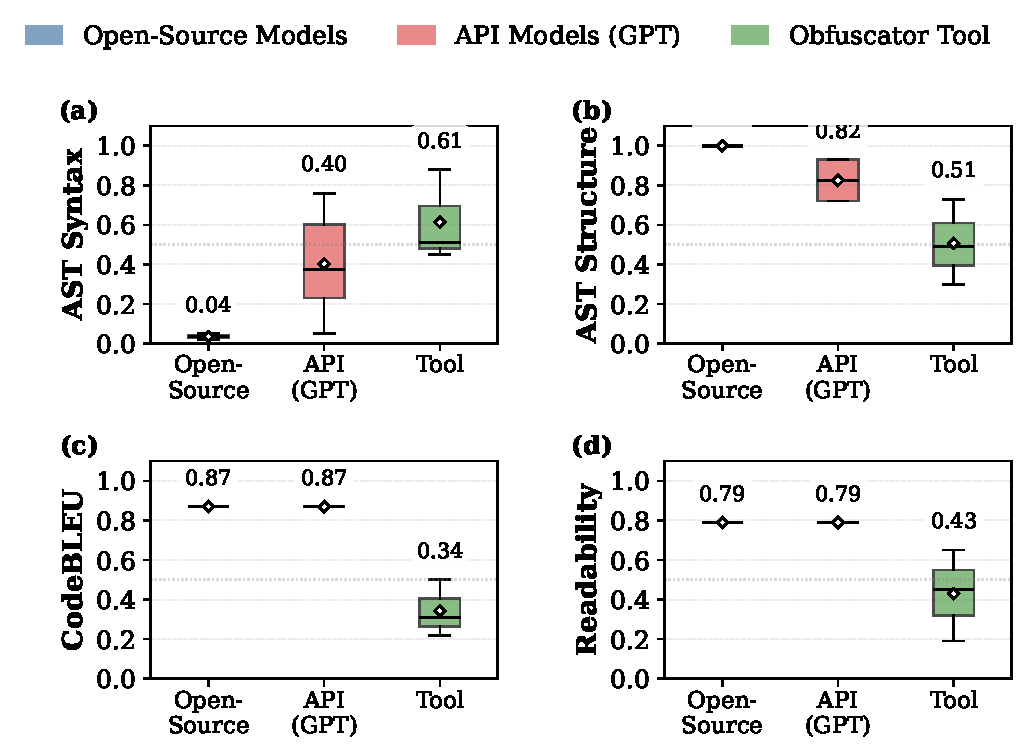
\includegraphics[width=.6\columnwidth, keepaspectratio]{figures/Result_figures/baseline_comparison_boxplot.pdf}
    \caption{Distribution of baseline performance across LLMs.% Open-source
    %models make little measurable change, GPT models make moderate lexical
    %changes, and the rule-based obfuscator produces large divergence from the
    %original program.
    }
    \label{fig:baseline_comparison}
    \vspace{-0.3cm}
\end{figure}




\textbf{Baseline reverse behavior.} We measure the reverse direction before any fine-tuning, so that the
post-fine-tuning reverse results have a point of comparison. 
% The two
The results indicate that they recover a measurable but partial
fraction of the original program on all three transformations.
For GPT-4.1-mini, $\text{Acc}_{\text{rev}}$ is 48.0\% on Identifier Renaming,
49.0\% on Dead Code Insertion, and 32.4\% on Literal Encryption.
GPT-3.5-Turbo reaches 40.2\%, 44.6\%, and 16.8\%.
Dead Code Insertion sits slightly above Identifier Renaming for both API models.
Literal Encryption remains lowest. 
As in the forward baseline, many unsuccessful cases fail at compilation, runtime, or test pass.
The recovery is moderate, not complete. It
registers as movement toward the original on the syntactic metrics
rather than as a return to the original program.
$\mathrm{Acc}_{\text{rev}}$ is decided per program against the tool references
above ($0.50$ / $0.33$ / $0.22$), not by comparing corpus-level means.
For GPT-4.1-mini, mean CodeBLEU of reverse outputs against the original is
$S(C_{\text{deobf}}, C_{\text{orig}}) = 0.440$ on Identifier Renaming,
$0.426$ on Dead Code Insertion, and $0.342$ on Literal Encryption.
Identifier-set overlap moves toward the original, with
$\text{AST}_{\text{synt}}$ gains of $+0.289$, $+0.214$, and $+0.194$.
The outputs sit between the tool-obfuscated input and the original code,
closer to the original but short of full restoration. 

The open-source models, consistent with their near-zero forward transformation at baseline, show negligible reverse recovery before fine-tuning as well. These results suggest that: these models may lack the instruction-following capacity to interpret the reverse prompt without task-specific context or the reverse transformation may exceed their zero-shot reasoning ability; or the scarcity of explicit deobfuscation examples in their pretraining data may make the mapping unrecognizable. Distinguishing these factors is left for future work.


% This reverse baseline uses the two API models, for which the inverse capability is measurable and the fine-tuning interface is controlled. The open-source models apply almost no transformation in either direction at baseline, as the forward results above show, so they provide a weaker reference point for the reverse comparison.






\subsection{Forward Performance After Standard Fine-Tuning}

% We then fine-tune each model on forward pairs and evaluate on the held-out
% ConDefects programs, to confirm that the models learn the forward transformation
% from the supervision they receive. \Cref{fig:model_performance} and
% \Cref{fig:sft_forward_performance} show that standard fine-tuning raises
% forward performance on all three transformations, with gains that vary by task
% type.

We then fine-tune each model with standard fine-tuning (SFT) on forward pairs
only. Each training example maps an original Java program to its
tool-obfuscated counterpart under one transformation type.
The instruction used during fine-tuning is
as follows:

\begin{tcolorbox}[colback=cyan!5, colframe=cyan!25, coltitle=black,
  title=Fine-Tuning Prompt Template, boxrule=0.4pt, left=2pt, right=2pt,
  top=2pt, bottom=2pt]
\small\texttt{Obfuscate the following Java code by \textit{<Obfuscation Technique>}
while preserving its functionality:}\\
\small\textbf{Input: \texttt{<Original code>}} \\
\small\texttt{Here's the obfuscated version preserving functionality:}\\
\small\textbf{Output: \texttt{<Obfuscated code>}}
\end{tcolorbox}

\noindent
Here \texttt{<Obfuscation Technique>} is Identifier Renaming, Dead Code
Insertion, or Literal Encryption. \texttt{<Original code>} is the input and
\texttt{<Obfuscated code>} is the expected tool output. After fine-tuning, we
evaluate on the held-out ConDefects programs with the same instruction format.
\Cref{fig:model_performance} and \Cref{fig:sft_forward_performance} show that
standard fine-tuning raises forward performance on all three transformations,
with gains that vary by task type.

The forward results follow a stable complexity ordering. Identifier Renaming is
learned best, at 68.9\% average success and 81.3\% for GPT-4.1-mini. Dead Code Insertion is harder, at 53.1\% average success and 72.7\% for Mistral. Literal Encryption is hardest, at 20.0\% average success and 29.7\% for Mistral. The ordering holds across models, which indicates that fine-tuning is most effective
when the target transformation reduces to local substitution and least effective
when it requires algorithmic manipulation of program values.

% Auto-correction raises forward results, and its benefit also shrinks with task
% complexity, at 17.6\% on Identifier Renaming, 18.2\% on Dead Code Insertion, and
% 10.1\% on Literal Encryption. The GPT models gain more than the open-source
% models, yet the task ordering is unchanged. An error analysis of the 2{,}805
% failed forward samples explains the pattern. Among them, 63\% compile and run but fail tests, 33\% crash at runtime, and 4\% fail to compile, so the dominant error
% mode is semantic rather than syntactic.


We then apply an iterative auto-correction loop to failed forward outputs.
When a generation fails to compile, execute, or pass tests, we feed the error
message back to the model with a correction prompt. We report results after
five iterations. Further iterations yield no additional gain under our setup.
The correction prompt is as follows:

\begin{tcolorbox}[colback=red!5, colframe=red!25, coltitle=black,
  title=Self-Correction Prompt, boxrule=0.4pt, left=2pt, right=2pt,
  top=2pt, bottom=2pt, fontupper=\small]
\textbf{System:} You are a code obfuscator. The previous obfuscated code did
not work. Here is the code and the error. Please correct the code so it
compiles and passes all tests.\\
\vspace{0.2cm}
\textbf{User:} \\
Original code (for reference):\\
\texttt{<Original Code>}\\
\vspace{0.1cm}
Previous obfuscated code:\\
\texttt{<Generated Code>}\\
\vspace{0.1cm}
Error message:\\
\texttt{<Compiler/Runtime Error or Failed Test Case>}\\
\vspace{0.1cm}
Please correct the code.
\end{tcolorbox}

\noindent
Auto-correction raises forward pass rates. The average gain is 16.6\% on
Identifier Renaming, 19.8\% on Dead Code Insertion, and 13.8\% on Literal
Encryption. GPT-3.5-Turbo rises from 76.3\% to 96.0\% on Identifier Renaming.
GPT-4.1-mini rises from 60.0\% to 88.7\% on Dead Code Insertion.
GPT-3.5-Turbo rises from 22.3\% to 46.7\% on Literal Encryption.
GPT models gain more than the open-source models on average
(20.8 percentage points versus 14.7 across the three transformations).
The gap is concentrated on Dead Code Insertion and Literal Encryption.
\Cref{fig:model_performance} reports the corrected pass rates.

% We measure the link between self-correction gain and transformation
% complexity with Spearman's rank correlation. The association is negative
% ($\rho = -0.85$, $p < 0.01$). 
Average gains stay high on Identifier Renaming
and Dead Code Insertion, where many failures are still recoverable from
compiler or test feedback. Gains shrink on Literal Encryption, where the
failure is usually a wrong program behavior rather than a fixable syntax
fault.
Under our setup, self-correction therefore repairs many surface errors.
It does not close the gap on Literal Encryption. The task
ordering after correction matches the ordering before correction.

We break down the 2{,}705 failed forward samples out of 5{,}400
evaluations.\footnote{Six models, three transformations, 300 evaluation
programs each.} Of these failures, 62\% compile and run but fail tests, 34\% crash at runtime, and
4\% fail to compile. \Cref{fig:errors_xp1} shows the distribution across
models and transformations. The pattern varies by task. On Identifier Renaming,
73\% of failures are incorrect outputs and 21\% are runtime crashes. On Dead
Code Insertion, incorrect outputs remain dominant at 69\%. On Literal
Encryption, runtime crashes rise to 45\% and incorrect outputs fall to 52\%.
Compilation failures stay low on every task (about 3\%--6\% of failures per
transformation). Models often emit code that looks well-formed, while they
still miss the required functional behavior. Appendix reports full details.


\begin{figure}[!ht]
    \centering
    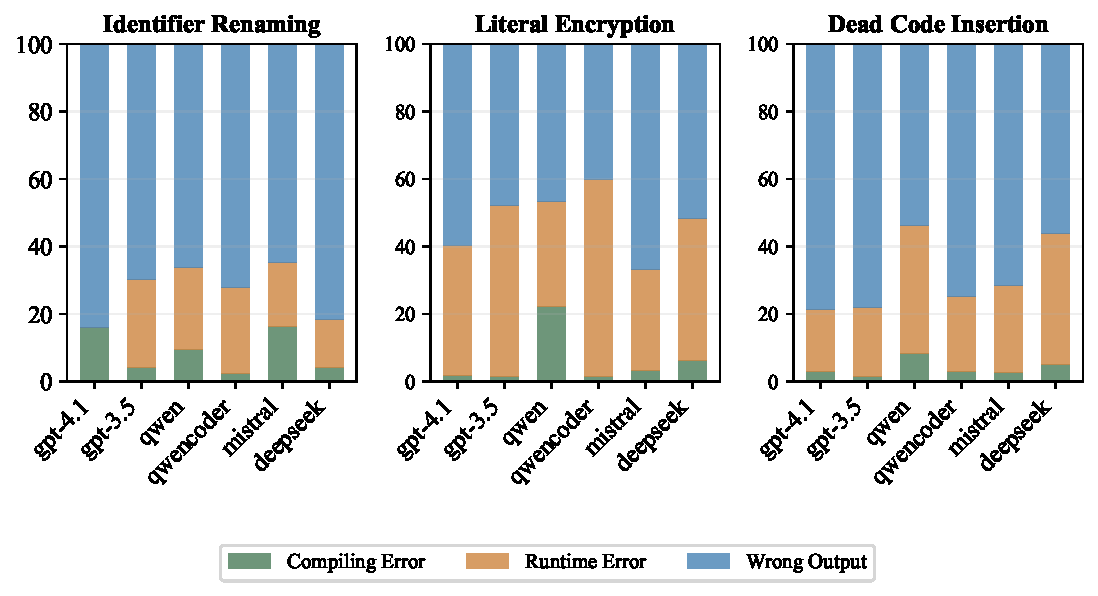
\includegraphics[width=.9\linewidth, height=5cm, keepaspectratio]{figures/figure_reversibility.pdf}
    \caption{Error-type distribution for failed forward outputs after SFT.
    Per-model bars keep the relative error profile of each model and are
    scaled so that each transformation matches the aggregate counts in
    Table~\ref{tab:error_distribution} (2{,}705 failures). Compilation
    failures are rare. Runtime crashes and incorrect outputs that still
    compile account for most failures.}
    \label{fig:errors_xp1}
\end{figure}


%%%%%%%%%%%%%%%%%%%%%%%%%%%%%%

The similarity metrics show that forward fine-tuning shifts model behavior in a
targeted way. On Identifier Renaming, $S(C_{\text{obf}},C_{\text{orig}})$ stays
between 0.42 and 0.50 while $S(C_{\text{obf}},C_{\text{tool}})$ stays between 0.49
and 0.51, a moderate lexical shift toward the tool pattern. On Dead Code
Insertion and Literal Encryption, $S(C_{\text{obf}},C_{\text{orig}})$ falls to
between 0.12 and 0.27 while $S(C_{\text{obf}},C_{\text{tool}})$ rises to between
0.59 and 0.73. Readability follows, from 0.79 on the original code to 0.57 on the
fine-tuned outputs. Standard fine-tuning thus teaches the forward surface pattern
even where full semantic fidelity is not reached.

\begin{figure}[h!]
    \centering
    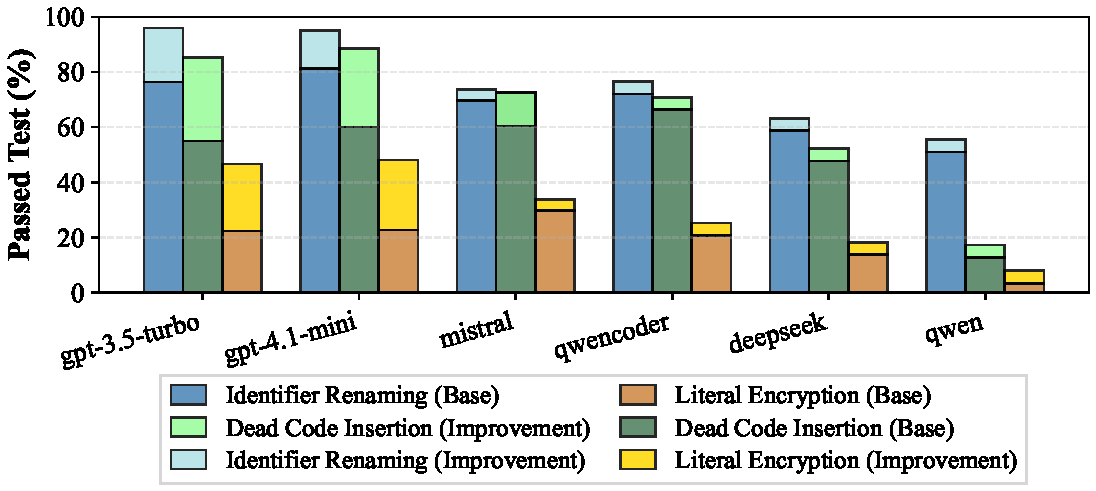
\includegraphics[width=.9\linewidth, height=4cm, keepaspectratio]{figures/model_performance_barplot.pdf}
    \caption{Fine-tuned LLM performance on forward obfuscation.}
    \label{fig:model_performance}
    \vspace{-3mm}
\end{figure}

\begin{figure}[!ht]
    \centering
    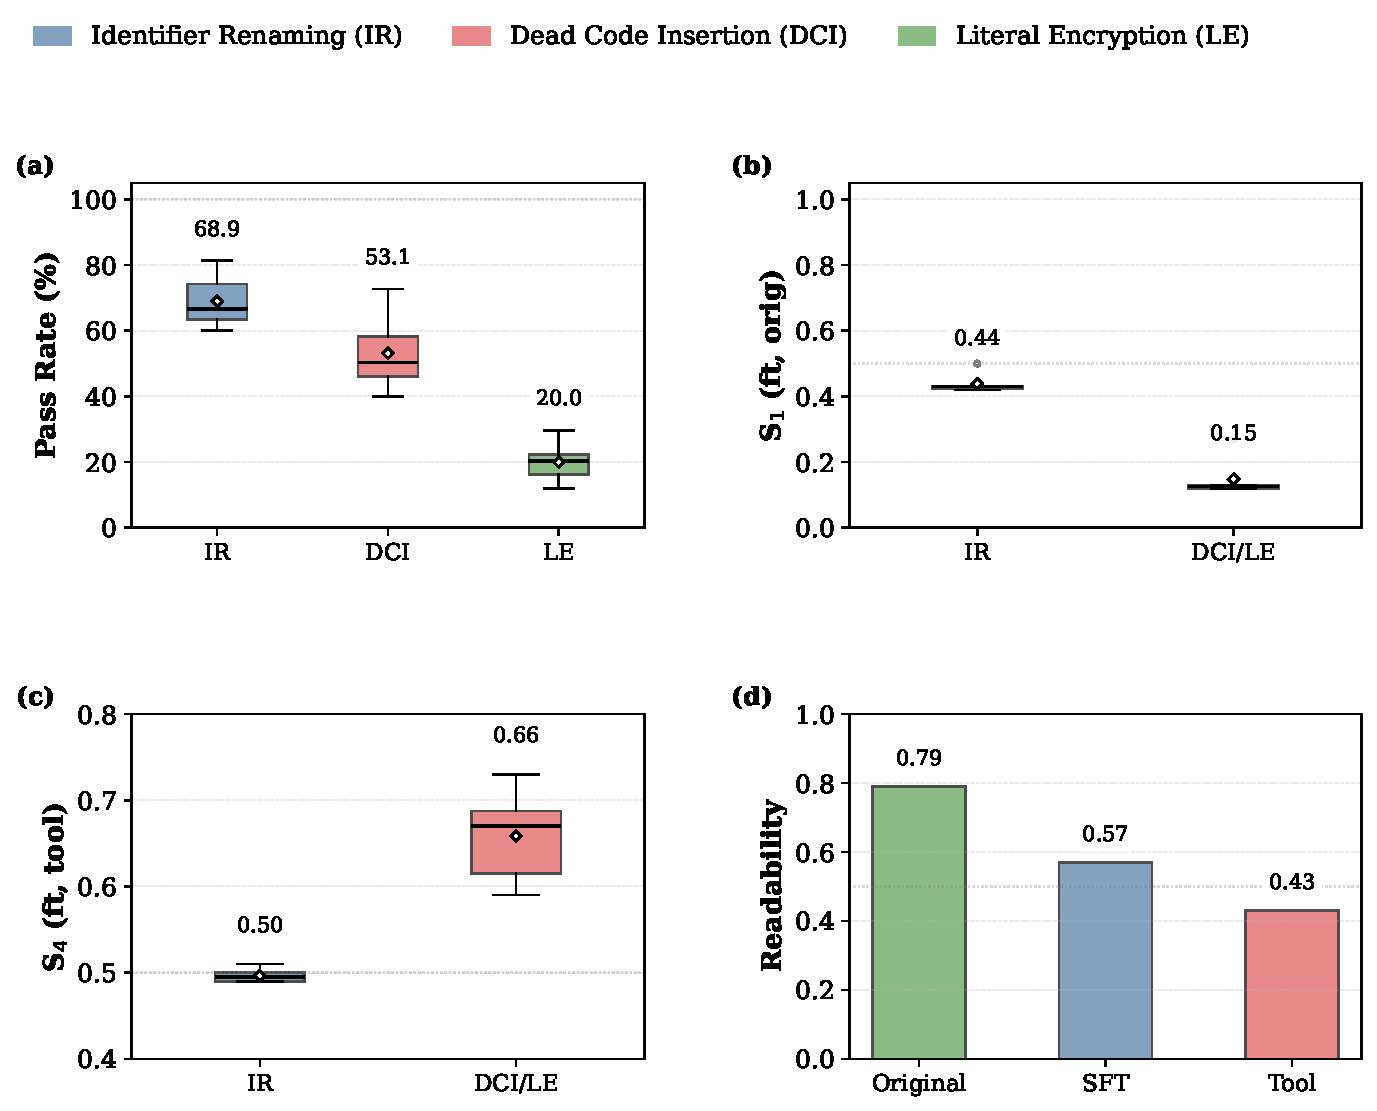
\includegraphics[width=.6\columnwidth, keepaspectratio]{figures/Result_figures/sft_forward_performance.pdf}
    \caption{Forward performance after standard fine-tuning. Pass rates and
    similarity trends show that models learn the forward syntactic pattern more
    reliably than they preserve semantic correctness on the harder tasks.}
    \label{fig:sft_forward_performance}
    \vspace{-0.25cm}
\end{figure}

\subsection{Reverse Evaluation with BRF}
\label{sec:reverse-eval}

%The reverse evaluation is the core result of the paper. 
We prompt every fine-tuned model to deobfuscate tool-generated obfuscated code under four strategies, namely direct instructions, few-shot prompting, chain-of-thought
prompting, and few-shot prompting combined with chain-of-thought. The appendix
lists the full prompts. If forward fine-tuning had preserved any usable inverse
capability, at least one of these strategies would yield outputs that move toward
the original program. None of them does.

Across all six models, all three transformations, and all four prompting
strategies, no output shows net positive movement on any evaluation channel
toward the original program. Reverse recovery is 0\% under the
$\mathrm{Acc}_{\text{rev}}$ rule. Against the reverse
baseline of Section~\ref{sec:baseline_experiment}, the unfine-tuned API
models succeed on 17\% to 49\% of evaluation programs under the same protocol.
This is a drop to zero. %, not a task that was out of reach to begin with. 
 The moderate deobfuscation present before fine-tuning disappears after forward-only
fine-tuning.

This zero is also not an artifact of the word ``deobfuscation''. A model
might fail a reverse prompt because it does not recognize the task label,
even if some inverse capability remained. As in the baseline wording check,
we therefore also prompt the fine-tuned models with reverse instructions that
never use that term. We ask them to restore meaningful identifier names, to
remove non-functional dead-code blocks, and to decrypt AES-encrypted literals
back to their original values. Under these formulations, the models still
emit code that is essentially identical to the obfuscated input. No
evaluation channel moves toward the original program. The result holds even
for Identifier Renaming, where reverse recovery was measurable before
fine-tuning (up to 48.0\% for GPT-4.1-mini). Prompt reformulation does not restore the inverse
mapping. The full prompts appear in the appendix.


%%%%%%%
The zero is not a collapse of generation. The reverse outputs pass the semantic
validity gate. They compile and preserve the behavior of the obfuscated input.
They fail because they do not move toward the original code.
On Identifier Renaming, $AST_{\text{synt}}$ stays near 0.01 against the
obfuscated input, so identifiers barely change.
$AST_{\text{struct}}$ stays at 1.0, so the control-flow skeleton is untouched
(Figure~\ref{fig:cognitive_specialization_fig}(b)).
Token counts move within 3\% of the obfuscated input.
These channels support near-verbatim reproduction of the obfuscated program.
CodeBLEU against the obfuscated input is lower, with
$S(C_{\text{deobf}},C_{\text{tool}})$ between 0.65 and 0.79.
Against the original, mean $S(C_{\text{deobf}},C_{\text{orig}})$ is 0.40 on
Identifier Renaming.
That value stays below the tool reference
$S(C_{\text{tool}},C_{\text{orig}})=0.50$.
On Dead Code Insertion and Literal Encryption, the same comparison uses the
tool references $0.33$ and $0.22$.
Under these references, CodeBLEU does not improve after SFT.
The remaining gap to the obfuscated input is consistent with formatting and
local edits that do not restore the original program.
Figure~\ref{fig:cognitive_specialization_fig}(a) shows the concentration near
the obfuscated endpoint across all three transformations.
Readability does not recover.
On Identifier Renaming, $R(C_{\text{deobf}})$ stays between 0.55 and 0.69,
below the original readability of 0.79.
Dead Code Insertion and Literal Encryption show no readability gain
(Figure~\ref{fig:cognitive_specialization_fig}(c)).

The AST and size metrics confirm that these outputs are near-verbatim
reproductions rather than failed deobfuscations. Across transformation types,
$AST_{\text{synt}}$ stays near 0.01, so identifiers remain almost unchanged,
and $AST_{\text{struct}}$ stays at 1.0, so the control-flow structure is
untouched (Figure~\ref{fig:cognitive_specialization_fig}(b)). Token counts move
within 3\% of the obfuscated input. Readability does not recover. On Identifier
Renaming, $R(C_{\text{deobf}})$ stays between 0.55 and 0.69, below the original
readability of 0.79, and Dead Code Insertion and Literal Encryption show no
readability gain (Figure~\ref{fig:cognitive_specialization_fig}(c)).

Prompting does not change the outcome. Few-shot examples and chain-of-thought
reasoning help when a model holds the underlying capability and needs better task
framing. Here they leave the direction of generation untouched.
Figure~\ref{fig:cognitive_specialization_fig}(d) shows that similarity to the
obfuscated input stays high under Simple, Few-Shot, CoT, and augmented prompts.
The models emit the obfuscated form even when the prompt requests the reverse,
and even when the reasoning trace has begun to describe the reverse mapping
(Figure~\ref{fig:cot_failure_main}). This persistence across prompt forms
separates a prompt mismatch from directional capability loss.

\begin{figure}[!ht]
    \centering
    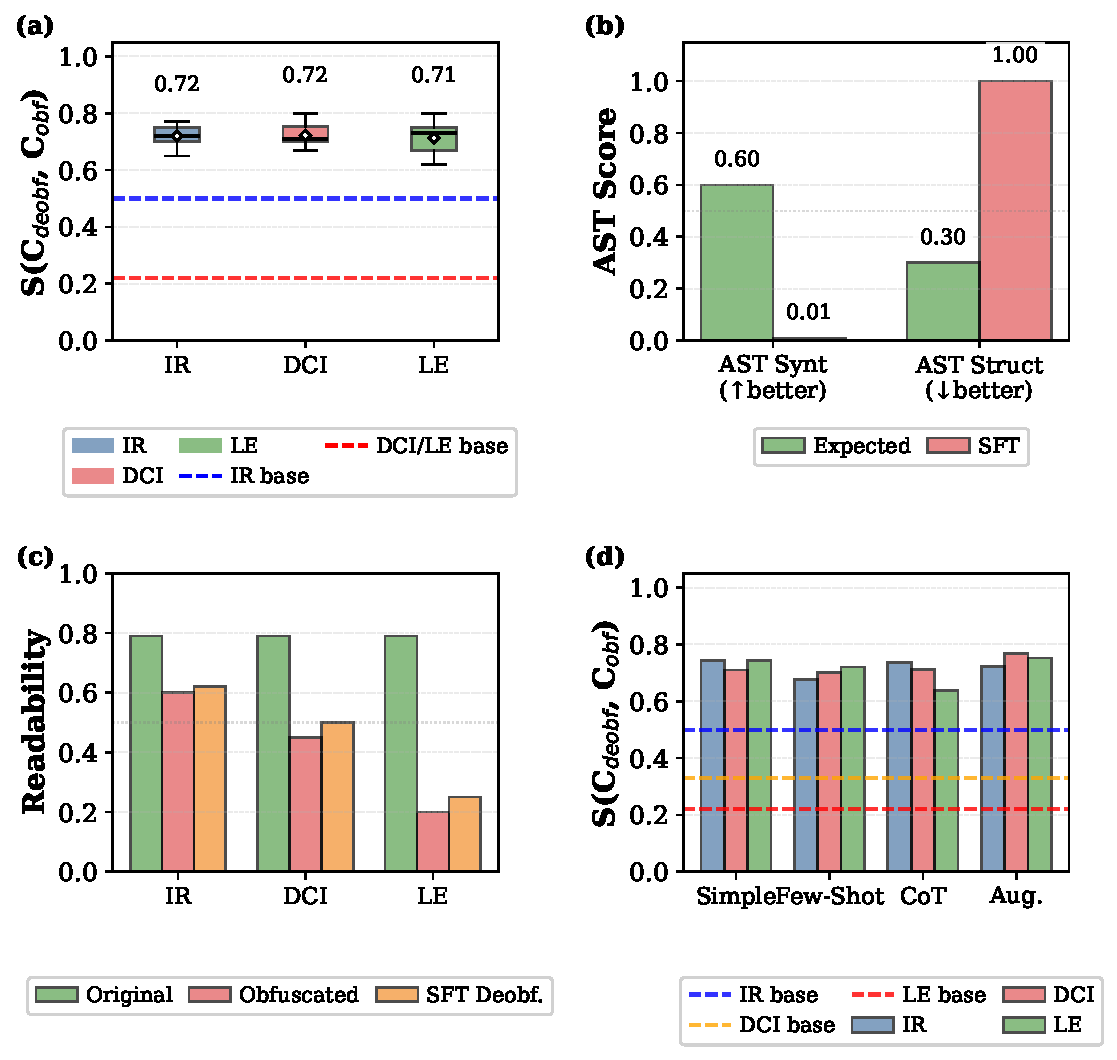
\includegraphics[width=.6\columnwidth, keepaspectratio]{figures/Result_figures/sft_reverse_cognitive_specialization.pdf}
    \caption{Reverse performance after standard fine-tuning. Across models and
    task types, outputs remain concentrated near the obfuscated endpoint instead
    of moving back toward the original program.}
    \label{fig:cognitive_specialization_fig}
\end{figure}

\begin{formal}
Standard fine-tuning creates a large bidirectional gap. The same models that
reach 12.0--81.3\% forward accuracy before self-correction produce 0\%
successful deobfuscation. Identifier, structure, and size metrics show
near-verbatim reproductions of the obfuscated input.
CodeBLEU stays closer to the obfuscated endpoint than to the original, without
reaching full token identity.
This is the defining behavioral signature of the inversion curse.
\end{formal}

\subsection{Directional Loss, Not Global Forgetting}
\label{sec:forgetting-probe}
A large forward-to-reverse gap admits two readings. Adaptation may have
suppressed the specific inverse of the trained transformation, or it may have
degraded the model broadly, in which case unrelated capabilities would fall
alongside the inverse. We separate the two by evaluating the
forward-obfuscation checkpoint, with no further fine-tuning, on its trained
inverse and on two tasks absent from the obfuscation corpus: Python-to-C
translation scored by re-execution, and MBPP code generation. All conditions
use identical prompts, decoding, and scoring.

\begin{table}[t]
\centering
\caption{Directional loss versus global forgetting. Forward-obfuscation
fine-tuning collapses the trained inverse while held-out capabilities stay
near baseline. Values are percentages; $\Delta$ in percentage points.}
\label{tab:forgetting-probe}
\begin{tabular}{@{}lccc@{}}
\toprule
Task & Baseline & Post-FT & $\Delta$ \\
\midrule
Reverse deobfuscation (Java)      & 48.0 & 0.0  & $-48.0$ \\
Python$\rightarrow$C (re-exec.)   & 26.8 & 22.0 & $-4.8$  \\
Code QA (MBPP)                    & 6.0  & 5.7  & $-0.3$  \\
\bottomrule
\end{tabular}
\vspace{-0.5cm}
\end{table}

The inverse collapses while the other tasks do not. Reverse deobfuscation
falls from 48.0\% to 0.0\% ($-48$ pp), whereas Python-to-C moves by $-4.8$ pp
and MBPP by $-0.3$ pp. Global forgetting would pull those two tasks down
together with the inverse. Instead the drop is confined to the direction paired
with the trained transformation. The failure is directional, which is what
separates the inversion curse from catastrophic forgetting and licenses the name.

\subsection{Translation and Compilation Checks}
\label{sec:transl-compil}

The two additional settings reproduce the directional trend under a lighter
protocol. For translation, forward-only fine-tuning on Python-to-Java lowers
Java-to-Python reverse accuracy from a baseline of 85.4\% to 63.3\%. For
compilation, forward-only fine-tuning on C-to-assembly lowers assembly-to-C
reverse accuracy from 16.5\% to 5.5\%. Allowing up to three generations raises translation reverse accuracy to 82.3\% (below the baseline pass@1), while the same allowance barely moves compilation reverse accuracy, at 8.5\%. The pass@3 gap between the two settings distinguishes degraded precision from
directional lock-in: the Java-to-Python capability is weakened but accessible
under repeated sampling, whereas assembly-to-C recovery is blocked regardless
of the number of attempts.

These checks carry less mechanistic detail than the obfuscation study, yet they
establish that the directional pattern is not confined to deobfuscation. The
milder loss under translation and the severe loss under compilation also track
the complexity ordering of the controlled testbed. Reverse performance degrades
less when the inverse approximates a constrained mapping between two high-level
languages, and more when it requires reconstruction from a lower-level
representation.

\section{Mechanism and Recovery Under Bidirectional Supervision}
\label{sec:cs_mechanism_section}

The previous section established what standard fine-tuning does. This section
asks why the reverse failure takes the form it does, and how much of it explicit
reverse supervision can repair. The evidence supports a deliberately narrow
claim. On lexical transformations the reverse mapping stays accessible at
inference time yet goes unused in the final generation. On harder
transformations, explicit reverse supervision restores structural rewriting but
not semantic recovery.

\subsection{Phenomenology of the Failure}
\label{sec:cs_phenomenology}

Three properties recur across the reverse evaluations. First, reverse recovery
falls to zero in every standard fine-tuning condition we test. Second, prompting
does not rescue the reverse direction. Third, the outputs concentrate at the
obfuscated endpoint rather than drifting randomly through program space. This
third property shows that the model has not become uncertain. It has
become directionally biased toward re-expressing the forward transformation.

The surface outcome is shared across task types, yet the inverse tasks differ in
difficulty. Identifier Renaming is local and lexical. Dead Code Insertion
requires the model to find and delete the semantically inert inserted blocks.
Literal Encryption requires recovery of hidden literal values from the inserted
decryption logic. We therefore read the uniform 0\% reverse recovery as a single
behavioral endpoint reached from increasingly different underlying difficulties.
The distinction returns when we compare recovery under bidirectional and
contrastive training.

For Identifier Renaming, the case for genuine capability loss is strongest.
Before fine-tuning, the GPT models already perform partial identifier
substitution in the forward direction. After standard fine-tuning, the same
models rename effectively in the forward direction yet fail entirely at reverse
restoration. The contrast is
not between a model that never had the reverse skill and one that still lacks it.
It is between a model family that manipulates identifiers in both directions at
baseline and the same family, after forward adaptation, locked into the trained
direction.

\subsection{Reasoning and Generation}
\label{sec:cs_mechanism}

The chain-of-thought probe supplies the most direct mechanism evidence. On
Identifier Renaming, a model states the correct reverse mapping in its reasoning
trace, for instance by noting that an obfuscated token should map back to a
meaningful identifier, and then returns the unchanged obfuscated code as its final
answer. The reasoning and the generation diverge, see Figure~\ref{fig:cot_failure_main}. We do not read the trace as a
faithful report of internal computation, since the faithfulness literature warns
against that reading~\cite{lanham2023measuring, turpin2023unfaithful}. We read it
more conservatively. The reverse mapping can be elicited in text while remaining
unused in the generated code.

%%%%%%%%%%%
\begin{figure}[!ht]
\centering
\definecolor{varRed}{HTML}{E74C3C}
\definecolor{varBlue}{HTML}{3498DB}
\definecolor{varGreen}{HTML}{2ECC71}
\begin{tcolorbox}[colback=gray!5, colframe=black!25, coltitle=black,
  title={\small\textbf{CoT Failure on Identifier Renaming (GPT-4.1-mini)}},
  boxrule=0.4pt, left=5pt, right=5pt, top=4pt, bottom=4pt, fontupper=\small]
\textbf{1.\ Obfuscated input:}
\begin{lstlisting}[language=Java, numbers=none, basicstyle=\small\ttfamily,
  aboveskip=2pt, belowskip=4pt, xleftmargin=0pt,
  emph={[1]l1l1l1}, emphstyle={[1]\colorbox{varRed!30}},
  emph={[2]l1l1l2}, emphstyle={[2]\colorbox{varBlue!30}},
  emph={[3]l1l1l3}, emphstyle={[3]\colorbox{varGreen!30}}]
public class Calculator {
    public static void main(String[] args) {
        int l1l1l1 = 10; int l1l1l2 = 20;
        int l1l1l3 = l1l1l1 + l1l1l2;
        System.out.println("The sum is: " + l1l1l3);
    }
}
\end{lstlisting}
\textbf{2.\ Model reasoning (correct):}
\begin{itemize}[leftmargin=*, topsep=1pt, itemsep=0pt]
  \item \texttt{l1l1l1}: stores first integer value $\to$ rename to \texttt{firstNumber}
  \item \texttt{l1l1l2}: stores second integer value $\to$ rename to \texttt{secondNumber}
  \item \texttt{l1l1l3}: stores the sum $\to$ rename to \texttt{sum}
\end{itemize}
\vspace{2pt}
\textbf{3.\ Final output (mapping ignored):}
\begin{lstlisting}[language=Java, numbers=none, basicstyle=\small\ttfamily,
  aboveskip=2pt, belowskip=2pt, xleftmargin=0pt,
  emph={[1]l1l1l1}, emphstyle={[1]\colorbox{varRed!30}},
  emph={[2]l1l1l2}, emphstyle={[2]\colorbox{varBlue!30}},
  emph={[3]l1l1l3}, emphstyle={[3]\colorbox{varGreen!30}}]
public class Calculator {
    public static void main(String[] args) {
        int l1l1l1 = 10; int l1l1l2 = 20;
        int l1l1l3 = l1l1l1 + l1l1l2;
        System.out.println("The sum is: " + l1l1l3);
    }
}
\end{lstlisting}
\end{tcolorbox}
\caption{GPT-4.1-mini model correctly identifies the reverse identifier mapping in its reasoning trace yet reproduces the obfuscated code verbatim in the final output, demonstrating the reasoning--generation disconnect. The full four-step trace appears in Appendix.}
\label{fig:cot_failure_main}
\end{figure}

%%%%%%%%%%

This behavior fits a generation-time directional bias. Standard fine-tuning
minimizes cross-entropy against forward obfuscated outputs, so the model is
rewarded for continuing the sequence in the forward direction rather than for
preserving a bidirectional relation between the original and transformed forms.
The probe does not establish the full mechanism. It does rule out the weakest
account, in which the model has lost the reverse association altogether, for the
lexical case.

\begin{figure*}[ht]
    \centering
    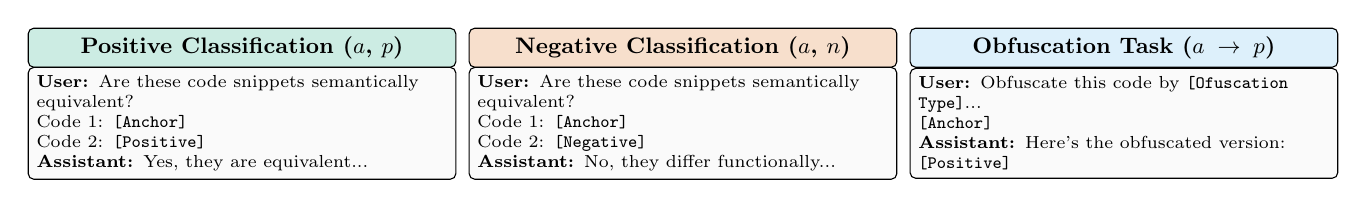
\begin{tikzpicture}[scale=0.8, every node/.style={scale=0.9}]
        \definecolor{poscolor}{RGB}{0,158,115}
        \definecolor{negcolor}{RGB}{213,94,0}
        \definecolor{gencolor}{RGB}{86,180,233}
        \definecolor{codebg}{RGB}{250,250,250}
        \definecolor{textgray}{gray}{0.15}

        % Positive Classification
        \node[draw, fill=poscolor!20, text width=5.8cm, align=center, font=\small\bfseries, rounded corners=2pt]
            at (-7, 5.2) {Positive Classification ($a$, $p$)};
        \node[draw, fill=codebg, text width=5.8cm, align=left, font=\scriptsize, rounded corners=2pt]
            at (-7, 4.0) {
            \textbf{User:} Are these code snippets semantically equivalent?\\
            Code 1: \texttt{[Anchor]}\\
            Code 2: \texttt{[Positive]}\\
            \textbf{Assistant:} Yes, they are equivalent...
        };

        % Negative Classification
        \node[draw, fill=negcolor!20, text width=5.8cm, align=center, font=\small\bfseries, rounded corners=2pt]
            at (0, 5.2) {Negative Classification ($a$, $n$)};
        \node[draw, fill=codebg, text width=5.8cm, align=left, font=\scriptsize, rounded corners=2pt]
            at (0, 4.0) {
            \textbf{User:} Are these code snippets semantically equivalent?\\
            Code 1: \texttt{[Anchor]}\\
            Code 2: \texttt{[Negative]}\\
            \textbf{Assistant:} No, they differ functionally...
        };

        % Forward Generation
        \node[draw, fill=gencolor!20, text width=5.8cm, align=center, font=\small\bfseries, rounded corners=2pt]
            at (7, 5.2) {Obfuscation Task ($a \rightarrow p$)};
        \node[draw, fill=codebg, text width=5.8cm, align=left, font=\scriptsize, rounded corners=2pt]
            at (7, 4.0) {
            \textbf{User:} Obfuscate this code by \texttt{[Ofuscation Type]}...\\
            \texttt{[Anchor]}\\
            \textbf{Assistant:} Here's the obfuscated version:\\
            \texttt{[Positive]}
        };
    \end{tikzpicture}
    \caption{The three distinct task formats used in Contrastive Fine-Tuning (CFT).}
    \label{fig:contrastive_prompting}
    \vspace{-0.45cm}
\end{figure*}

Whether the same reasoning-generation split holds for Dead Code Insertion and
Literal Encryption remains open. Those tasks demand more than token-level
substitution, and our prompts do not surface comparably explicit intermediate
mappings. The mechanism claim is therefore scoped. The lexical evidence is
direct, while the extension to structural and semantic inverses rests on the
shared behavioral endpoint together with the differing recovery profiles reported
next.


\subsection{Balanced Bidirectional Fine-Tuning}
\label{sec:bft}



Balanced bidirectional fine-tuning (BFT) trains on forward and reverse pairs at
once and therefore sets a recovery ceiling for the reverse task. Its results show
that standard fine-tuning does not erase reverse capability in any absolute
sense. Given explicit reverse supervision, the models recover much of the inverse
on Identifier Renaming and Dead Code Insertion. On the lexical transformation,
BFT reaches up to 80\% recovery, at a 59\% average across models. On the
structural transformation, it reaches 76\% at best, at a 52\% average.


The recovery registers on every reverse-direction metric. Against the SFT
endpoint, BFT raises identifier-set overlap with the original to 0.45.
It lowers $AST_{\text{struct}}$ between the deobfuscated output and the
obfuscated input to 0.37.
The outputs therefore move away from the obfuscated input and toward the
original code in both identifiers and structure. CodeBLEU and readability follow.
Readability rises by 0.29 in absolute terms over the SFT reverse output.
It does not reach the original readability of 0.79. BFT thus demonstrates
that the reverse task is not inherently impossible on the lexical and structural
cases, and that explicit reverse supervision re-opens that direction.



% Literal Encryption resists this treatment. Even with balanced reverse
% supervision, its reverse recovery stays at 0\%. We therefore treat Literal
% Encryption as a boundary case for the current methods rather than as evidence for
% a single mechanism. The failure could stem from the difficulty of autoregressive
% recovery of encrypted literals, from the enlarged inverse search space, or from a
% deeper interaction between fine-tuning and sequence generation. The defensible
% conclusion is operational. For data-flow inverses of this kind, explicit reverse
% supervision is insufficient under the present setup.


Literal Encryption resists this treatment. Even with balanced reverse
supervision, its reverse recovery stays at 0\%.
Under this task design, that endpoint is expected.
The model must recover AES-encrypted literals from hard-coded decryption
logic, not apply a local inverse mapping.
We therefore treat Literal Encryption as a semantic boundary case for the
current methods, not as proof of a generic reverse failure.
The defensible conclusion is operational.
For semantic inverses of this kind, explicit reverse supervision is
insufficient under the present setup.


\begin{table}[tb]
\centering
\caption{Consolidated reverse accuracies (\%) and forward accuracies in
parentheses across models, training strategies, and transformation types.
SFT (Fwd) is the forward pass rate before self-correction.
Post-correction rates appear in Section~\ref{sec:cognitive_specialization}
and Figure~\ref{fig:model_performance}.
$\Delta_{\text{BRF}}$ is the bidirectional gap under each strategy.}
\begin{adjustbox}{width=.7\columnwidth,center}
\label{tab:consolidated_results}
\begin{tabular}{@{}l cc cc cc cc@{}}
\toprule
& \multicolumn{2}{c}{\textbf{SFT}} & \multicolumn{2}{c}{\textbf{BFT}} & \multicolumn{2}{c}{\textbf{CFT}} & \multicolumn{2}{c}{$\Delta_{\text{BRF}}$} \\
\cmidrule(lr){2-3} \cmidrule(lr){4-5} \cmidrule(lr){6-7} \cmidrule(lr){8-9}
\textbf{Model} & Rev & (Fwd) & Rev & (Fwd) & Rev & (Fwd) & SFT & CFT \\
\midrule
\multicolumn{9}{l}{\textit{Identifier Renaming (IR)}} \\
\midrule
GPT-4.1-mini & 0 & (81) & 80 & (72) & 52 & (72) & 81 & 20 \\
GPT-3.5-Turbo & 0 & (76) & 72 & (70) & 48 & (68) & 76 & 20 \\
Qwen2.5-7B & 0 & (60) & 52 & (58) & 39 & (60) & 60 & 21 \\
Qwen2.5-Coder-7B & 0 & (65) & 55 & (64) & 43 & (65) & 65 & 22 \\
DeepSeek-R1-Distill-Qwen-7B & 0 & (63) & 48 & (56) & 36 & (56) & 63 & 20 \\
Mistral-7B & 0 & (68) & 49 & (60) & 41 & (62) & 68 & 21 \\
\midrule
\multicolumn{9}{l}{\textit{Dead Code Insertion (DCI)}} \\
\midrule
GPT-4.1-mini & 0 & (60) & 76 & (65) & 0 & (68) & 60 & 68 \\
GPT-3.5-Turbo & 0 & (53) & 58 & (62) & 0 & (60) & 53 & 60 \\
Qwen2.5-7B & 0 & (40) & 42 & (40) & 0 & (38) & 40 & 38 \\
Qwen2.5-Coder-7B & 0 & (48) & 45 & (44) & 0 & (46) & 48 & 46 \\
DeepSeek-R1-Distill-Qwen-7B & 0 & (45) & 38 & (38) & 0 & (34) & 45 & 34 \\
Mistral-7B & 0 & (73) & 55 & (52) & 0 & (52) & 73 & 52 \\
\midrule
\multicolumn{9}{l}{\textit{Literal Encryption (LE)}} \\
\midrule
GPT-4.1-mini & 0 & (22) & 0 & (28) & 0 & (26) & 22 & 26 \\
GPT-3.5-Turbo & 0 & (22) & 0 & (40) & 0 & (38) & 22 & 38 \\
Qwen2.5-7B & 0 & (12) & 0 & (14) & 0 & (12) & 12 & 12 \\
Qwen2.5-Coder-7B & 0 & (19) & 0 & (16) & 0 & (16) & 19 & 16 \\
DeepSeek-R1-Distill-Qwen-7B & 0 & (15) & 0 & (12) & 0 & (10) & 15 & 10 \\
Mistral-7B & 0 & (30) & 0 & (20) & 0 & (18) & 30 & 18 \\
\bottomrule
\end{tabular}
\end{adjustbox}
\end{table}

\section{Contrastive Fine-Tuning as a Probe}
\label{contrastive}


BFT shows what happens when reverse supervision is made explicit. Contrastive
fine-tuning poses a different question. Can reverse capability be recovered
without reverse labels, provided the training objective preserves semantic
proximity between original and obfuscated programs? We treat CFT as a mechanistic
probe, not as a production recipe. If directional capability loss has a
representational component, then a forward-only objective augmented with semantic
contrast should reduce that component on at least the simpler inverses.



CFT adds a contrastive objective to the forward generation loss. Each training
example contains an anchor program, its obfuscated counterpart as a positive
example, and an unrelated program as a negative example, see Figure~\ref{fig:contrastive_prompting}. The model is optimized
to generate the forward transformation while distinguishing semantically related
from unrelated pairs. Following prior contrastive learning formulations~\cite{chen2020simple,
he2020momentum},~\cite{jain2021contracode, li2022coderetriever} the combined loss is

\begin{equation}
\mathcal{L}_{\text{CFT}} = \lambda_1 \mathcal{L}_{\text{gen}} + \lambda_2(\mathcal{L}_{\text{pos}} + \mathcal{L}_{\text{neg}}),
\end{equation}

with $\lambda_1 = \lambda_2 = 1$ in our open-source runs. The salient property of
this objective is that CFT never observes a reverse label. Any recovery in the
reverse direction must therefore arise from preserving semantic structure while
the model learns the forward transformation.

% \begin{figure*}[!ht]
%     \centering
%     \begin{tikzpicture}[scale=0.9, every node/.style={scale=0.9}]
%         \definecolor{poscolor}{RGB}{0,158,115}
%         \definecolor{negcolor}{RGB}{213,94,0}
%         \definecolor{gencolor}{RGB}{86,180,233}
%         \definecolor{codebg}{RGB}{250,250,250}
%         \definecolor{textgray}{gray}{0.15}

%         % Positive Classification
%         \node[draw, fill=poscolor!20, text width=5cm, align=center, font=\small\bfseries, rounded corners=2pt]
%             at (-7, 6.2) {Positive Classification ($a$, $p$)};
%         \node[draw, fill=codebg, text width=5.8cm, align=left, font=\scriptsize, rounded corners=2pt]
%             at (-7, 4.5) {
%             \textbf{User:} Are these code snippets semantically equivalent?\\
%             Code 1: \texttt{[Anchor]}\\
%             Code 2: \texttt{[Positive]}\\
%             \textbf{Assistant:} Yes, they are equivalent...
%         };

%         % Negative Classification
%         \node[draw, fill=negcolor!20, text width=5.8cm, align=center, font=\small\bfseries, rounded corners=2pt]
%             at (0, 6.2) {Negative Classification ($a$, $n$)};
%         \node[draw, fill=codebg, text width=5.8cm, align=left, font=\scriptsize, rounded corners=2pt]
%             at (0, 4.5) {
%             \textbf{User:} Are these code snippets semantically equivalent?\\
%             Code 1: \texttt{[Anchor]}\\
%             Code 2: \texttt{[Negative]}\\
%             \textbf{Assistant:} No, they differ functionally...
%         };

%         % Forward Generation
%         \node[draw, fill=gencolor!20, text width=5.8cm, align=center, font=\small\bfseries, rounded corners=2pt]
%             at (7, 6.2) {Obfuscation Task ($a \rightarrow p$)};
%         \node[draw, fill=codebg, text width=5.8cm, align=left, font=\scriptsize, rounded corners=2pt]
%             at (7, 4.5) {
%             \textbf{User:} Obfuscate this code by \texttt{[Ofuscation Type]}...\\
%             \texttt{[Anchor]}\\
%             \textbf{Assistant:} Here's the obfuscated version:\\
%             \texttt{[Positive]}
%         };

%         % Learning Objectives
%         \draw[->, thick, poscolor] (-7, 3.4) -- (-7, 3.0);
%         \node[font=\normalsize, poscolor] at (-7, 2.8) {$\mathcal{L}_{pos}$: Minimize semantic distance};

%         \draw[->, thick, negcolor] (0, 3.4) -- (0, 3.0);
%         \node[font=\normalsize, negcolor] at (0, 2.8) {$\mathcal{L}_{neg}$: Maximize semantic distance};

%         \draw[->, thick, gencolor] (7, 3.4) -- (7, 3.0);
%         \node[font=\normalsize, gencolor] at (7, 2.8) {$\mathcal{L}_{gen}$: Learn transformation};

%         % Combined Loss
%         \node[draw, fill=white, rounded corners=3pt, text width=6cm, align=left, font=\large] 
%             at (0, 2) {$\mathcal{L}_{\text{CFT}} = \lambda_1 \mathcal{L}_{pos} + \lambda_2 \mathcal{L}_{neg} + \mathcal{L}_{gen}$};
%     \end{tikzpicture}
%     \caption{Contrastive Fine-Tuning prompting strategy.
%     %The anchor ($a$) is paired with a semantically equivalent transformation ($p$) and a dissimilar variant ($n$). The model learns to minimize semantic distance for $(a, p)$, maximize it for $(a, n)$, and generate $p$ from $a$.
%     }
%     \label{fig:contrastive_prompting}
% \end{figure*}

%%%%%%%%%%%%%%%%%%%%%%%%%%%%%%%%%%%%%%%%%%%%%%%%%%%

% \begin{figure*}[!ht]
%     \centering
%     \begin{tikzpicture}[scale=0.9, every node/.style={scale=0.9}]
%         \definecolor{poscolor}{RGB}{0,158,115}
%         \definecolor{negcolor}{RGB}{213,94,0}
%         \definecolor{gencolor}{RGB}{86,180,233}
%         \definecolor{codebg}{RGB}{250,250,250}
%         \definecolor{textgray}{gray}{0.15}

%         % Positive Classification
%         \node[draw, fill=poscolor!20, text width=5cm, align=center, font=\small\bfseries, rounded corners=2pt]
%             at (-7, 5.2) {Positive Classification ($a$, $p$)};
%         \node[draw, fill=codebg, text width=5.8cm, align=left, font=\scriptsize, rounded corners=2pt]
%             at (-7, 4.2) {
%             \textbf{User:} Are these code snippets semantically equivalent?\\
%             Code 1: \texttt{[Anchor]}\\
%             Code 2: \texttt{[Positive]}\\
%             \textbf{Assistant:} Yes, they are equivalent...
%         };

%         % Negative Classification
%         \node[draw, fill=negcolor!20, text width=5.8cm, align=center, font=\small\bfseries, rounded corners=2pt]
%             at (0, 5.2) {Negative Classification ($a$, $n$)};
%         \node[draw, fill=codebg, text width=5.8cm, align=left, font=\scriptsize, rounded corners=2pt]
%             at (0, 4.2) {
%             \textbf{User:} Are these code snippets semantically equivalent?\\
%             Code 1: \texttt{[Anchor]}\\
%             Code 2: \texttt{[Negative]}\\
%             \textbf{Assistant:} No, they differ functionally...
%         };

%         % Forward Generation
%         \node[draw, fill=gencolor!20, text width=5.8cm, align=center, font=\small\bfseries, rounded corners=2pt]
%             at (7, 5.2) {Obfuscation Task ($a \rightarrow p$)};
%         \node[draw, fill=codebg, text width=5.8cm, align=left, font=\scriptsize, rounded corners=2pt]
%             at (7, 4.2) {
%             \textbf{User:} Obfuscate this code by \texttt{[Ofuscation Type]}...\\
%             \texttt{[Anchor]}\\
%             \textbf{Assistant:} Here's the obfuscated version:\\
%             \texttt{[Positive]}
%         };

%         % Learning Objectives
%         \draw[->, thick, poscolor] (-7, 3.3) -- (-7, 3.0);
%         \node[font=\normalsize, poscolor] at (-7, 2.6) {$\mathcal{L}_{pos}$: Minimize semantic distance};

%         \draw[->, thick, negcolor] (0, 3.3) -- (0, 3.0);
%         \node[font=\normalsize, negcolor] at (0, 2.6) {$\mathcal{L}_{neg}$: Maximize semantic distance};

%         \draw[->, thick, gencolor] (7, 3.3) -- (7, 3.0);
%         \node[font=\normalsize, gencolor] at (7, 2.6) {$\mathcal{L}_{gen}$: Learn transformation};

%         % Combined Loss
%         \node[draw, fill=white, rounded corners=3pt, text width=6cm, align=left, font=\large] 
%             at (0, 1.5) {$\mathcal{L}_{\text{CFT}} = \lambda_1 \mathcal{L}_{pos} + \lambda_2 \mathcal{L}_{neg} + \mathcal{L}_{gen}$};
%     \end{tikzpicture}
%     \caption{Contrastive Fine-Tuning prompting strategy.
%     %The anchor ($a$) is paired with a semantically equivalent transformation ($p$) and a dissimilar variant ($n$). The model learns to minimize semantic distance for $(a, p)$, maximize it for $(a, n)$, and generate $p$ from $a$.
%     }
%     \label{fig:contrastive_prompting}
% \end{figure*}

%%%%%%%%%%%%%%%%%%%%%%%%%



% \begin{figure}[!ht]
%     \centering
%     \scriptsize
%     \begin{tikzpicture}[
%         node distance=0.5cm,
%         codebox/.style={rectangle, rounded corners=3pt, draw=black!40, line width=0.8pt, 
%                         fill=white, drop shadow={opacity=0.15}, 
%                         minimum height=0.8cm, align=left},
%         arrow/.style={-{Stealth[length=2mm]}, line width=1.2pt}
%     ]
    
%     % Configure Java syntax highlighting
%     \lstset{
%         language=Java,
%         basicstyle=\ttfamily\fontsize{7}{8}\selectfont,
%         keywordstyle=\color{blue!70!black}\bfseries,
%         identifierstyle=\color{black},
%         numbers=none,
%         breaklines=true,
%         xleftmargin=3pt,
%         xrightmargin=3pt,
%         backgroundcolor=\color{gray!5},
%         frame=none,
%         escapechar=@,
%         columns=flexible
%     }
    
%     % SFT: Obfuscated Input → Verbatim Reproduction (Left)
%     \node[codebox, draw=red!50, text width=0.45\columnwidth] (sft) {
%         \textbf{\footnotesize SFT: Cognitive Specialization}\\
%         \textit{\tiny Obfuscated input reproduced verbatim}\\[2pt]
%         \begin{lstlisting}
% public class Main_2 {
%   void solve() {
%     Scanner @\colorbox{red!20}{\texttt{IlIlIllIlIlI}}@ = 
%       new Scanner(System.in);
%     int @\colorbox{red!20}{\texttt{llIlIIlIIl}}@ = 
%       @\colorbox{red!20}{\texttt{IlIlIllIlIlI}}@.nextInt();
%     for (int i = @\colorbox{red!20}{\texttt{llIlIIlIIl}}@;
%          i >= 0; --i)
%       System.out.println(i);
%   }
% }
%         \end{lstlisting}
%         \vspace{2pt}
%         \textcolor{red!70!black}{\tiny\bfseries \ding{55} AST$_{\text{synt}}$ = 0.999 (99\% identifiers retained)}
%     };
    
%     % CFT: Successful Deobfuscation (Right)
%     \node[codebox, draw=green!50!black, text width=0.45\columnwidth, right=0.5cm of sft] (cft) {
%         \textbf{\footnotesize CFT: Emergent Bidirectionality}\\
%         \textit{\tiny Semantic recovery with readable identifiers}\\[2pt]
%         \begin{lstlisting}
% public class @\colorbox{green!20}{\texttt{CountingNumbers}}@ {
%   void @\colorbox{green!20}{\texttt{countDown}}@() {
%     Scanner @\colorbox{green!20}{\texttt{scanner}}@ =
%       new Scanner(System.in);
%     int @\colorbox{green!20}{\texttt{number}}@ = 
%       @\colorbox{green!20}{\texttt{scanner}}@.nextInt();
%     for (int i = @\colorbox{green!20}{\texttt{number}}@;
%          i >= 0; --i)
%       System.out.println(i);
%   }
% }
%         \end{lstlisting}
%         \vspace{2pt}
%         \textcolor{green!60!black}{\tiny\bfseries \checkmark AST$_{\text{synt}}$ = 0.17 (83\% identifiers changed)}
%     };
    
%     \end{tikzpicture}
    
%     \caption{Cognitive Specialization vs. Emergent Bidirectionality.}
%     \label{fig:cognitive_specialization}
% \end{figure}


%%%%%%%%%%%%%%%%%%%%%%%%%%%%%%%%%%%%%%%%%%%%%%%%%%


% \begin{figure}[!ht]
%     \centering
%     \scriptsize
%     \begin{tikzpicture}[
%         node distance=0.5cm,
%         codebox/.style={rectangle, rounded corners=3pt, draw=black!40, line width=0.8pt, 
%                         fill=white, drop shadow={opacity=0.15}, 
%                         minimum height=0.8cm, align=left},
%         arrow/.style={-{Stealth[length=2mm]}, line width=1.2pt}
%     ]
    
%     % Configure Java syntax highlighting
%     \lstset{
%         language=Java,
%         basicstyle=\ttfamily\fontsize{7}{8}\selectfont,
%         keywordstyle=\color{blue!70!black}\bfseries,
%         identifierstyle=\color{black},
%         numbers=none,
%         breaklines=true,
%         xleftmargin=3pt,
%         xrightmargin=3pt,
%         backgroundcolor=\color{gray!5},
%         frame=none,
%         escapechar=@,
%         columns=flexible
%     }
    
%     % SFT: Obfuscated Input → Verbatim Reproduction (Left)
%     \node[codebox, draw=red!50, text width=0.45\columnwidth] (sft) {
%         \textbf{\footnotesize SFT: Cognitive Specialization}\\
%         \textit{\tiny Obfuscated input reproduced verbatim}\\[2pt]
%         \begin{lstlisting}
% public class Main_2 {
%   void solve() {
%     Scanner @\colorbox{red!20}{\texttt{IlIlIllIlIlI}}@ = 
%       new Scanner(System.in);
%     int @\colorbox{red!20}{\texttt{llIlIIlIIl}}@ = 
%       @\colorbox{red!20}{\texttt{IlIlIllIlIlI}}@.nextInt();
%     for (int i = @\colorbox{red!20}{\texttt{llIlIIlIIl}}@;
%          i >= 0; --i)
%       System.out.println(i);}
% }
%         \end{lstlisting}
%         \vspace{2pt}
%         \textcolor{red!70!black}{\tiny\bfseries \ding{55} AST$_{\text{synt}}$ = 0.999 (99\% identifiers retained)}
%     };
    
%     % CFT: Successful Deobfuscation (Right)
%     \node[codebox, draw=green!50!black, text width=0.45\columnwidth, right=0.5cm of sft] (cft) {
%         \textbf{\footnotesize CFT: Emergent Bidirectionality}\\
%         \textit{\tiny Semantic recovery with readable identifiers}\\[2pt]
%         \begin{lstlisting}
% public class @\colorbox{green!20}{\texttt{CountingNumbers}}@ {
%   void @\colorbox{green!20}{\texttt{countDown}}@() {
%     Scanner @\colorbox{green!20}{\texttt{scanner}}@ =
%       new Scanner(System.in);
%     int @\colorbox{green!20}{\texttt{number}}@ = 
%       @\colorbox{green!20}{\texttt{scanner}}@.nextInt();
%     for (int i = @\colorbox{green!20}{\texttt{number}}@;
%          i >= 0; --i)
%       System.out.println(i);}
% }
%         \end{lstlisting}
%         \vspace{2pt}
%         \textcolor{green!60!black}{\tiny\bfseries \checkmark AST$_{\text{synt}}$ = 0.17 (83\% identifiers changed)}
%     };
    
%     \end{tikzpicture}
    
%     \caption{Cognitive Specialization vs. Emergent Bidirectionality.}
%     \label{fig:cognitive_specialization}
% \end{figure}


%%%%%%%%%%%%%%%%%%%%%%%%%%%%%%%%%%%%%%%%%%%%%


\begin{figure}[!ht]
  \centering
  \scriptsize
  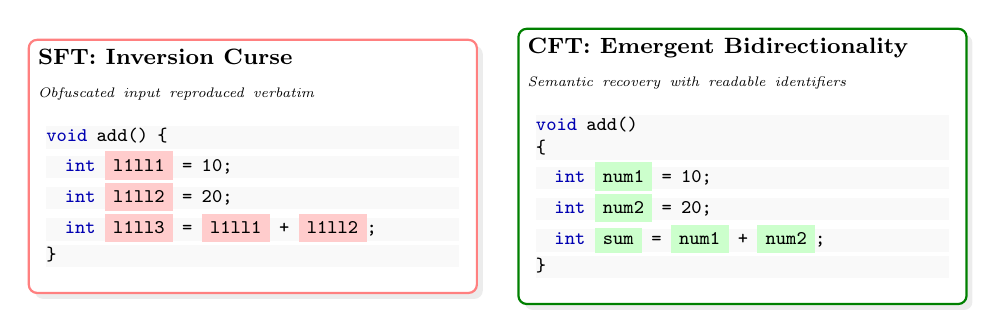
\begin{tikzpicture}[
      node distance=0.5cm,
      codebox/.style={rectangle, rounded corners=3pt, draw=black!40, line width=0.8pt, 
                      fill=white, drop shadow={opacity=0.15}, 
                      minimum height=0.8cm, align=left},
      arrow/.style={-{Stealth[length=2mm]}, line width=1.2pt}
  ]
  
  % Configure Java syntax highlighting
  \lstset{
      language=Java,
      basicstyle=\ttfamily\fontsize{7}{8}\selectfont,
      keywordstyle=\color{blue!70!black}\bfseries,
      identifierstyle=\color{black},
      numbers=none,
      breaklines=true,
      xleftmargin=3pt,
      xrightmargin=3pt,
      backgroundcolor=\color{gray!5},
      frame=none,
      escapechar=@,
      columns=flexible
  }
  
  % SFT: Obfuscated Input → Verbatim Reproduction (Left)
  \node[codebox, draw=red!50, text width=0.45\columnwidth] (sft) {
      \textbf{\footnotesize SFT: Inversion Curse}\\
      \textit{\tiny Obfuscated input reproduced verbatim}\\[2pt]
      \begin{lstlisting}
void add() {
  int @\colorbox{red!20}{\texttt{l1ll1}}@ = 10;
  int @\colorbox{red!20}{\texttt{l1ll2}}@ = 20;
  int @\colorbox{red!20}{\texttt{l1ll3}}@ = @\colorbox{red!20}{\texttt{l1ll1}}@ + @\colorbox{red!20}{\texttt{l1ll2}}@;
}
      \end{lstlisting}
%      \vspace{2pt}
%      \textcolor{red!70!black}{\tiny\bfseries \ding{55} AST$_{\text{synt}}$ = 0.999 (99\% identifiers retained)}
  };
  
  % CFT: Successful Deobfuscation (Right)
  \node[codebox, draw=green!50!black, text width=0.45\columnwidth, right=0.5cm of sft] (cft) {
      \textbf{\footnotesize CFT: Emergent Bidirectionality}\\
      \textit{\tiny Semantic recovery with readable identifiers}\\[2pt]
      \begin{lstlisting}
void add() 
{
  int @\colorbox{green!20}{\texttt{num1}}@ = 10;
  int @\colorbox{green!20}{\texttt{num2}}@ = 20;
  int @\colorbox{green!20}{\texttt{sum}}@ = @\colorbox{green!20}{\texttt{num1}}@ + @\colorbox{green!20}{\texttt{num2}}@;
}
      \end{lstlisting}
%      \vspace{2pt}
 %     \textcolor{green!60!black}{\tiny\bfseries \checkmark AST$_{\text{synt}}$ = 0.17 (83\% identifiers changed)}
  };
  
  \end{tikzpicture}
  \caption{Inversion     Curse vs. Emergent Bidirectionality.}
  \label{fig:cognitive_specialization}
  % \vspace{-0.6cm}
\end{figure}

The outcome is task dependent. CFT keeps forward accuracy close to SFT, at a 64\%
average and 72\% for GPT-4.1-mini, while raising reverse recovery on Identifier
Renaming from 0\% to between 36\% and 52\% across models, for a 43\% average. On
Dead Code Insertion and Literal Encryption, reverse recovery stays at 0\%, as
under SFT. CFT recovers part of the inverse only where the reverse mapping is
local enough for representation-level alignment to take effect.

The metric profile on Identifier Renaming matches that reading.
Identifier-set overlap with the original rises to 0.83.
The outputs therefore move close to the original identifier set.
Readability on Identifier Renaming rises from $R(C_{\text{tool}})=0.65$ to
$R(C_{\text{deobf}})=0.74$, near the original readability of 0.79.
The forward-reverse gap contracts from a complete collapse under SFT to about 21
points under CFT on Identifier Renaming (Table~\ref{tab:consolidated_results}).
The recovery is incomplete, yet it exceeds any plausible noise.
See Figure~\ref{fig:cft_emergent_bidirectionality}.


Read alongside BFT, CFT supports a two-component account of the failure. On the
lexical transformation, part of the loss is representational and can be reduced
without reverse labels. On the structural and semantic transformations,
representation-level alignment is not enough, which points to a heavier
generative burden once the inverse demands statement deletion or algorithmic
recovery. CFT does not solve directional capability loss in general. It locates
where the failure is partly geometric and where it is governed by sequence
generation under an asymmetric objective, example is shown in Figure~\ref{fig:cognitive_specialization}.

\begin{figure}[!ht]
    \centering
    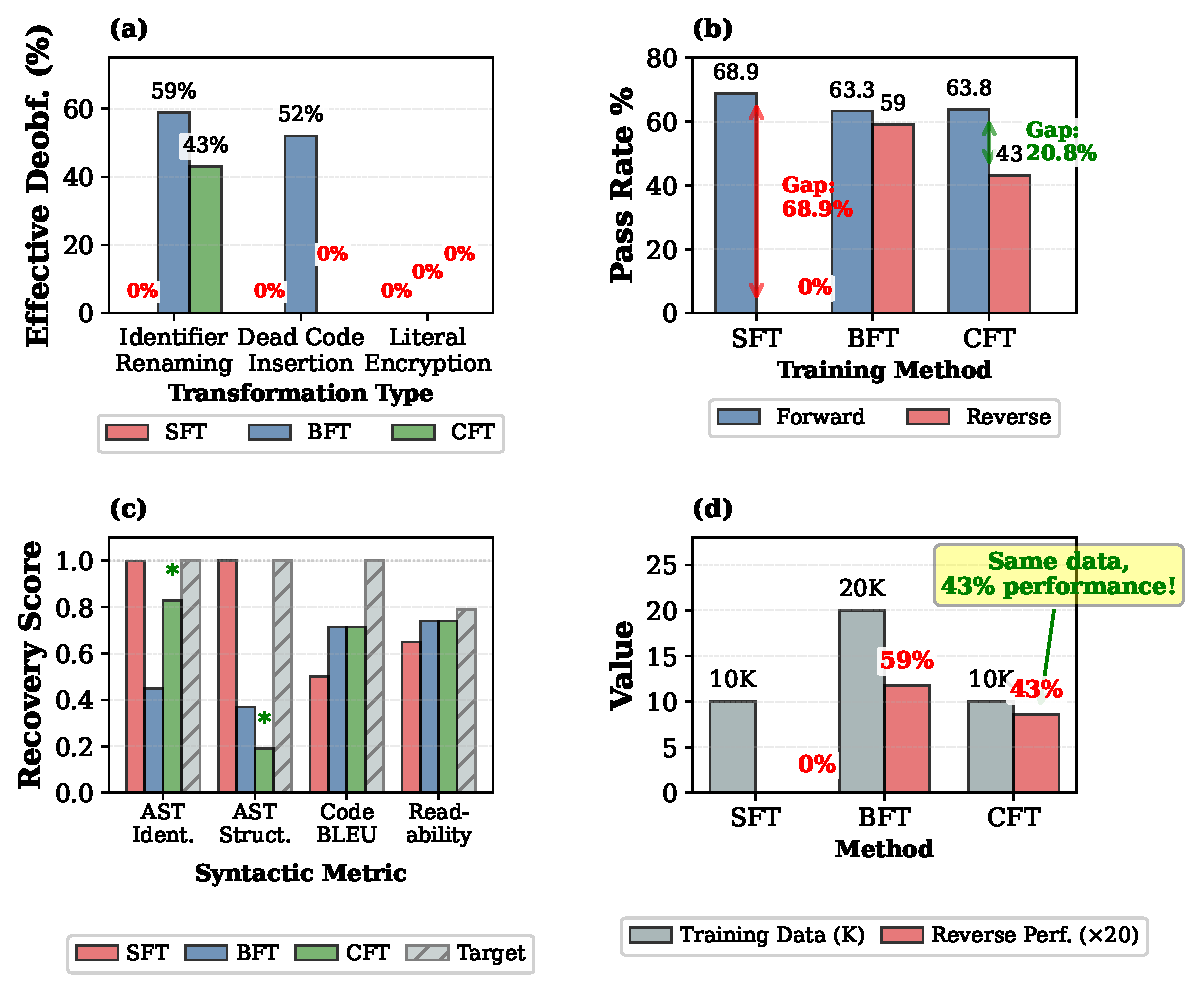
\includegraphics[width=.6\columnwidth, keepaspectratio]{figures/Result_figures/cft_emergent_bidirectionality.pdf}
    \caption{Contrastive fine-tuning partially restores bidirectionality on
    Identifier Renaming but not on the structural or semantic tasks.}
    \label{fig:cft_emergent_bidirectionality}
    \vspace{-0.5cm}
\end{figure}


\section{Related Work}
\label{sec:related}

\subsection{Directional Asymmetry in Language Models}
\label{sec:rw-reversal}

Autoregressive models can learn a relation in one direction without learning its reverse: a model trained on ``A is B'' often fails to answer ``B is A''~\cite{berglund2024reversal, grosse2023influence}.
Lv et al. attribute this reversal curse to the next-token objective, which maximizes $p(b \mid a)$ but offers no guarantee on $p(a \mid b)$~\cite{lv2024reversal}, while Wang and Sun trace it to the way transformers represent concepts~\cite{wang2025binding}.
Remedies generally expose the model to both directions during training, either by adding reversed strings to the data~\cite{golovneva2024reverse} or, as in back-translation and its use in TransCoder for code, by generating training pairs from the reverse direction~\cite{sennrich2016backtranslation, lachaux2021unsupervised}.

These studies concern facts or training pairs with a single correct reverse answer.
The inverse tasks we study are executable procedures whose outputs can be tested and admit many correct forms (Definition~\ref{def:pair}), so we score progress toward the source rather than exact recovery.
We also shift the question from pretraining to downstream fine-tuning.
Our balanced bidirectional fine-tuning (Section~\ref{sec:bft}) is close in intent to reverse training, but relies on explicit inverse pairs rather than reversed strings.

\subsection{Side Effects of Fine-Tuning}
\label{sec:rw-forgetting}

Sequential training has been known to overwrite earlier knowledge~\cite{mccloskey1989catastrophic, french1999catastrophic}, and regularization and distillation methods were designed to limit this forgetting~\cite{kirkpatrick2017overcoming, li2018lwf}.
In code models, replay and regularization reduce forgetting under API drift~\cite{weyssow2023continual}, and parameter-efficient methods such as LoRA forget less than full fine-tuning~\cite{biderman2024lora}.
Kotha et al. propose a complementary account in which fine-tuning shifts the task a model infers from its prompt, so that a disguised prompt can restore abilities that appeared lost~\cite{kotha2024implicit}.
Beyond forgetting, fine-tuning can also produce side effects outside the target task, including weaker safety alignment~\cite{qi2024finetuning} and broad misalignment~\cite{betley2025emergent}.

These studies measure tasks unrelated to the fine-tuning objective.
We instead measure its inverse, which shares inputs, outputs, and vocabulary with the trained task, and we use unrelated tasks only as a control for general forgetting.% (Section~\ref{sec:forgetting}).
The account of Kotha et al. is relevant here, since a fine-tuned model may interpret a reverse prompt as a forward request.
We do not evaluate replay or regularization. They remain candidate mitigations outside this study.

\subsection{Code LLMs on Paired Tasks}
\label{sec:rw-paired}

LLMs are now applied to each side of the pairs we study.
They translate code, although their translations can introduce bugs~\cite{pan2024lost, yang2024unitrans}, and they are used to decompile binaries~\cite{tan2024llm4decompile, hu2024degpt} and to obfuscate code~\cite{mohseni2025obfuscate}.
Each of these studies evaluates the direction it targets.
Other work exploits both directions for evaluation: round-trip correctness runs a model forward and backward to check its outputs without labels~\cite{allamanis2024roundtrip}, and CRUXEval asks models to predict outputs from inputs as well as inputs from outputs~\cite{gu2024cruxeval}.
Semantics-preserving transformations are also used to probe the robustness of code models~\cite{yefet2020adversarial, rabin2021generalizability} and to build positive pairs for contrastive learning~\cite{jain2021contracode}.

These works either evaluate a fixed model or ask whether a prediction remains stable under a transformation.
Our question is whether a model can still undo a transformation after it has learned to apply it.
BRF addresses this question by comparing both directions before and after fine-tuning and by reporting the change as a regression.
Our contrastive fine-tuning reuses the positive-pair idea of ContraCode, but only as a probe (Section~\ref{contrastive}) and not as a training recipe.

\subsection{Faithfulness of Reasoning Traces}
\label{sec:rw-faithfulness}

A generated explanation need not reflect the computation behind an answer~\cite{jacovi2020faithfulness}, and chain-of-thought text can misrepresent the actual reason for a prediction~\cite{turpin2023unfaithful, lanham2023measuring}.
We therefore treat reasoning traces as behavioral evidence only (Section~\ref{sec:cs_mechanism}) and make no claim about internal representations.

\medskip
In summary, prior work has studied directional asymmetry on facts, forgetting on unrelated tasks, and the bidirectional use of models that were not adapted to one direction.
Our study connects these lines for paired code transformations, within the scope of one controlled testbed and two additional settings, and with behavioral evidence on mechanism.
\section{Threats to Validity}
\label{sec:threats}

\subsection{Internal Validity}

% \textit{Alternative explanation of the reverse failure.}
% A fine-tuned model may infer a forward task from any Java input~\cite{kotha2024implicit}.
% It would then ignore the reverse instruction.
% Three observations limit this threat.
% First, the reverse outputs keep the size and structure of the obfuscated input.
% A model that re-applied the forward transformation would insert more dead code or encrypt more literals.
% Second, the reasoning trace on Identifier Renaming follows the reverse instruction.
% Third, held-out tasks lose less than the inverse with the same checkpoint.
% These observations do not fully separate the two explanations.
% Our definition of the effect is behavioral.
% Both explanations describe a model that keeps the trained direction under a reverse prompt.

\textit{Alternative explanation of the reverse failure.}
The reverse failure may not reflect a lost capability.
After fine-tuning, the model may simply infer the forward task from any Java input and ignore the reverse instruction~\cite{kotha2024implicit}.
Under this explanation, the failure would concern instruction following rather than the inverse itself.
Three observations argue against it.
First, a model that re-applied the forward transformation would change the obfuscated input further, for instance by inserting more dead code or encrypting more literals.
The reverse outputs show no such change, since they keep the size and structure of the obfuscated input (Section~\ref{sec:reverse-eval}).
Second, on Identifier Renaming, the reasoning trace follows the reverse instruction and proposes the correct mapping, even though the final output leaves the code unchanged (Section~\ref{sec:cs_mechanism}).
The model therefore reads the reverse request, but does not act on it.
Third, with the same checkpoint, unrelated tasks lose far less than the inverse, which suggests that instruction following is largely preserved.
These observations weaken the alternative explanation.
%A control that gives other Java tasks to the fine-tuned models would separate the two accounts.
This limit does not affect our main claim, because we define the inversion curse by behavior rather than by cause.
Both accounts describe a model that stays in the trained direction under a reverse prompt, so the alternative explanation is a possible cause of the effect.

\textit{Training configuration.}
The reverse failure could result from overly aggressive training rather than from forward fine-tuning itself.
We limit this risk in two ways.
First, we selected the training size and schedule through a preliminary study, and we kept the configuration with the best forward performance.
Second, we used standard LoRA settings for 7B models~\cite{hu2022lora} and the provider settings for the API models.
We did not sweep learning rates or LoRA ranks, and a milder configuration might reduce the loss.
The reverse failure nevertheless appears in both training regimes, with 1,000 pairs for the API models and 10,000 pairs for the open-source models.
These regimes also differ in model family and optimizer, so this comparison does not isolate the effect of training size.

\textit{Prompt sensitivity.}
Other prompts might elicit the inverse.
We tested four prompting strategies.
They include few-shot examples and chain-of-thought.
None restored the reverse direction after fine-tuning.

\textit{Data contamination.}
% Pretraining data may contain the evaluation programs.
% We evaluate on ConDefects~\cite{condefects}. % [EXISTING]
% This dataset was built to reduce leakage concerns.
% Contamination would also affect the baseline and the fine-tuned model alike.
% It cannot by itself produce a drop after fine-tuning.
% \textit{Data contamination.}
To limit contamination between adaptation and evaluation, we fine-tune on CodeNet and evaluate on ConDefects dataset.
Both datasets may nevertheless appear in the pretraining data of the models.
We reduce this risk on the fine-tuning side by generating the training pairs with an obfuscator.
The obfuscated programs are produced for this study, so their exact form is unlikely to occur in pretraining data.
Our results also vary with the transformation type and the training strategy, which points to an effect of adaptation on obfuscated data rather than to recall of memorized programs.

\subsection{Construct Validity}

% \textit{Reverse recovery criterion.}
% Our criterion counts any positive movement toward the source on any channel.
% This choice accepts many valid deobfuscations (Definition~\ref{def:pair}).
% It may also count small changes as recoveries.
% The baseline reverse rates may therefore overstate full recovery.
% This leniency does not weaken the post-fine-tuning result.
% Under the same lenient criterion, no fine-tuned configuration recovers any program.
% We also report the per-channel similarity values.
% Readers can thus judge the size of each change.

\textit{Reverse recovery criterion.}
Evaluating deobfuscation is a challenge.
Tests can confirm that an output preserves the behavior of the program, but the obfuscated input already passes the same tests.
Deciding whether an output is actually deobfuscated therefore requires syntactic measures, and to our knowledge no single metric establishes this in a systematic way.
We therefore use four complementary channels, each capturing a different aspect of recovery.
An output counts as a recovery if it is valid and moves closer to the original, and we read the channels together to judge how consistent a change is.
This broad rule accepts the many valid forms of a deobfuscated program, but it also counts small, partial changes.

\textit{Semantic equivalence.}
We use test suites as the oracle of equivalence.
Tests cannot cover every behavior.
Each evaluation program comes with an average of 16 tests.
Test-based equivalence is standard in code generation and translation studies~\cite{pan2024lost}.

\textit{Similarity and readability metrics.}
CodeBLEU, AST overlap, and readability metrics are proxies for recovery.
As mention before, no single metric captures deobfuscation quality.
We therefore combine several independent channels.
The readability model was built from human judgments~\cite{scalabrino2018readability}. 

\textit{Reasoning traces.}
Chain-of-thought text may not reflect the computation behind an answer~\cite{turpin2023unfaithful,jacovi2020faithfulness}.
We use traces as behavioral evidence only.
We make no claim about internal representations.

\subsection{External Validity}

\textit{Language and transformations.}
The main study uses Java programs and three obfuscation types from one tool.
These types cover lexical, structural, and data-flow transformations, and they match techniques observed in real Android apps~\cite{dong2018android, wermke2018obfuscation}.
They do not cover all existing techniques.
Industrial obfuscators also apply transformations such as control-flow flattening and reflection~\cite{dong2018android}, which we leave for future work.
Our programs are also file-level, and they do not fully reflect real-world code such as Android applications or multi-file repositories.
Such systems involve dependencies across files and often exceed the context size of current LLMs, which prevented us from evaluating them.
The translation and compilation checks extend the observation to two other paired tasks, but each check uses a single model, so their results are indicative.

\textit{Models.}
\label{sec:models-ttv}
We acknowledge that our study does not include current state-of-the-art models. Two constraints explain this choice.
First, fine-tuning access to proprietary models is limited.
%Anthropic does not offer it on its own platform~\cite{aws2024haikufinetuning}.
%Google restricts it to selected Gemini versions~\cite{google2026geminituning}.
OpenAI offers it for a few models only~\cite{azure2026finetuning}.

Second, recent open-weight models are far larger than the models we fine-tuned.
Table~\ref{tab:open-sizes} lists examples.
Only a fraction of their weights is active for each token.
Fine-tuning still requires the full set of weights in memory.
% At 16-bit precision, each parameter takes two bytes.
% The smallest model in Table~\ref{tab:open-sizes} thus needs about 460\,GB for its weights alone.
% A 7B model needs about 14\,GB.
LoRA reduces the number of trainable parameters~\cite{hu2022lora},
%QLoRA reduces memory through quantization~\cite{dettmers2023qlora}. % [EXISTING]
but does not remove the need to load the base model.
%This requirement exceeds our academic hardware. 
The smallest model in Table~\ref{tab:open-sizes} thus needs about 460\,GB for its weights alone.

\begin{table}[t]
\centering
\caption{Size of recent open-weight models. Memory is the approximate size of the weights at 16-bit precision (2 bytes per parameter).}
\label{tab:open-sizes}
\small
\begin{tabular}{lrrr}
\toprule
Model & Total & Active & Weights (16-bit) \\
\midrule
DeepSeek-V4-Pro~\cite{deepseek2026v4} & 1.6T & 49B & $\approx$3.2\,TB \\
Kimi K2~\cite{kimi2025k2} & 1T & 32B & $\approx$2.0\,TB \\
GLM-5~\cite{glm2026glm5} & 744B & 40B & $\approx$1.5\,TB \\
Mistral Large 3~\cite{mistral2025large3} & 675B & 41B & $\approx$1.35\,TB \\
Qwen3.5-397B-A17B~\cite{qwen2026qwen35} & 397B & 17B & $\approx$0.8\,TB \\
MiniMax-M2~\cite{minimax2026m2} & 230B & 10B & $\approx$460\,GB \\
\midrule
7B model (this study) & 7B & 7B & $\approx$14\,GB \\
\bottomrule
\end{tabular}
\end{table}

Our results may therefore not directly generalize to these models.
However, the effect appears in both open-source evaluated models and proprietary models, far larger (GPT series).
This suggests that the effect is not specific to open 7B models under LoRA.
%It does not show that the effect holds for current frontier models.

We also do not evaluate agentic systems.
Such systems use a model together with tools, whereas fine-tuning adapts the model itself, which is the object of our study.
An agent built on a model that has lost the inverse may inherit this limitation, although tools may compensate for part of it.

\textit{Adaptation methods.}
We study LoRA and provider fine-tuning.
Other adaptation methods exist, such as full fine-tuning and continual-learning methods like replay or EWC~\cite{kirkpatrick2017overcoming, weyssow2023continual}.
We therefore do not claim that our findings generalize to all these methods.


\section{Discussion}
\label{sec:discussion}

The principal implication is methodological. Forward-only evaluation can certify
a fine-tuned model that has quietly lost capability on the inverse task. In
software engineering that risk spans more than one benchmark. Developers move
between paired tasks such as translation and back-translation and compilation and
decompilation. Mutation and repair raise a similar operational risk.
They fall outside Definition~\ref{def:pair}, because a mutant changes program
behavior. A pipeline that checks only the trained direction can promote the model variant that is least reliable once the workflow demands reversal, inspection, or rollback.

The risk extends beyond obfuscation. Security workflows couple forward and
reverse transformations, and recent work delegates both decompilation and
obfuscation to language models~\cite{tan2024llm4decompile, mohseni2025obfuscate}.
Modernization workflows do the same for translation, where forward translations
already carry functional bugs~\cite{pan2024lost, eniser2024rust}. Our checks on
translation and compilation show the same directional loss in those domains. The
governing claim concerns validation discipline. When a deployment context
contains a meaningful inverse task, that inverse must be evaluated in its own
right.

The mechanism evidence warrants a narrow reading. On Identifier Renaming, the
chain-of-thought probe agrees with a reasoning-generation gap. The model surfaces
the reverse identifier mapping yet generates the obfuscated code unchanged. The
behavior fits an account in which standard fine-tuning strengthens a forward
generation prior more than it preserves the bidirectional relation between source
and transformed code. The lexical result does not establish this as the sole
mechanism, and we do not claim that it carries unchanged to the harder tasks.

The recovery results fix the limits of what can be concluded. BFT shows that the
reverse direction is not inherently unreachable on the lexical and structural
tasks. Explicit supervision restores much of $\mathrm{Acc}_{\text{rev}}$ on
Identifier Renaming and Dead Code Insertion. CFT shows that part of the lexical
loss is recoverable without reverse labels, which points to a representational
component. Literal Encryption bounds these interventions. Full reverse
supervision fails there, so the present evidence cannot reduce the phenomenon to
one cause. The defensible summary is that directional capability loss interacts
with task complexity, and that the interaction becomes severe once the inverse
demands algorithmic recovery.

BRF follows from this finding as an instrument rather than a theory of model
cognition. It is a low-cost diagnostic that asks whether adaptation to a forward
transformation has introduced a hidden regression in the reverse direction. The
logic is the logic of regression testing. A local improvement is not sufficient
evidence of system reliability when the same change can break another part of the
workflow, and bidirectional evaluation supplies the missing check.

Several threats to validity remain. The main experiments use Java and six
decoder-only models, which limits the external validity of the exact percentages.
We mitigate this by spanning open and proprietary models and by adding the
translation and compilation checks. The strongest evidence of genuine capability
loss appears on Identifier Renaming, where the GPT models show measurable
baseline transformation ability and lose the reverse direction after standard
fine-tuning. On the harder tasks, the data supports the behavioral claim of
directional collapse more firmly than the stronger claim that an
already-demonstrated reverse skill was destroyed.

The study also stops short of direct representation analysis. We do not measure
internal geometry, activation dynamics, or decoding-time competition between
forward and reverse continuations, and those analyses are the natural next step.
Evaluation on encoder-decoder models, retrieval-augmented systems, and hybrid
symbolic-neural pipelines is also needed. The present results justify that
effort, since fine-tuning can reshape a code model in a directionally asymmetric
way that ordinary evaluation leaves invisible.

\section{Conclusion}
\label{sec:conclusion}

Forward fine-tuning can create a hidden failure mode in code LLMs. In our
controlled testbed, the adaptation step that raises forward obfuscation accuracy from below 5\%
to between 12.0\% and 81.3\% before self-correction,  depending on transformation type, drives down reverse deobfuscation accuracy to 0\%. The reverse
outputs remain executable and semantically valid, yet they stay near-verbatim
reproductions of the obfuscated input rather than steps back toward the original
readable program. 
% Forward success therefore does not entail preservation of the
% inverse capability.
Forward success, therefore, does not preserve the inverse capability.

The recovery experiments qualify that claim. Balanced bidirectional supervision
restores much of the reverse performance on the lexical and structural tasks,
while contrastive fine-tuning restores the lexical inverse without reverse
labels. Literal Encryption resists all three strategies. The translation and
compilation settings reproduce the directional trend outside the primary
obfuscation study. When a fine-tuned code LLM is destined for a setting in which
the inverse transformation matters, that inverse should be evaluated in its own
right, and BRF exposes the capability loss that forward-only benchmarks miss.

\noindent\textbf{Data Availability.} Code, datasets, and evaluation results are available at
\url{https://anonymous.4open.science/r/Bidirectional_Reasoning_Framework-B111/README.md}


%\balance
% \bibliographystyle{IEEEtran}
% \bibliography{references}


\bibliographystyle{ACM-Reference-Format}
%\bibliography{sample-base}
%\bibliographystyle{plain}
\bibliography{references}

\clearpage
\appendix
% \clearpage
\section{Transformation Taxonomy}
\label{appendix:taxonomy}

\begin{table*}[htbp]
\centering
\caption{Taxonomy of Code Transformations and Their Cognitive Demands}
\label{tab:transformation_taxonomy}
\begin{adjustbox}{width=.75\linewidth,center}
\begin{tabularx}{\textwidth}{@{}l|l|X|X|X@{}}
\toprule
\textbf{Transformation Type} & \textbf{Level} & \textbf{Transformation Description} & \textbf{Reverse Task Goal} & \textbf{Cognitive Challenge} \\ \midrule
Identifiers Renaming\\(Variable, Class, Methods) & Lexical & Replaces meaningful identifiers with obfuscated names (e.g., \texttt{TotalNum} $\rightarrow$ \texttt{IILLLL}). & Generate readable, semantically appropriate identifiers (e.g., \texttt{Sum}, \texttt{x}). & Requires abstraction over identifier roles and naming conventions. \\ \addlinespace
Dead Code Insertion & Structural & Injects non-functional or misleading code blocks (e.g., \texttt{if (false) \{...\}}). & Remove irrelevant code while preserving original logic. & Requires distinguishing functional vs. non-functional code paths. \\ \addlinespace
Literals Encryption & Semantic & Encrypts literals (strings, integers) and embeds decryption logic within the code. & Replace encrypted literals with interpretable, semantically equivalent values. & Requires reasoning over encrypted values and the embedded decryption behavior. \\ \bottomrule
\end{tabularx}
\end{adjustbox}
\noindent\textit{Note:} For the \textbf{Identifier Renaming} transformation, all identifiers are replaced with visually similar patterns such as \texttt{IILLLL}, \texttt{IILL}, etc.
\end{table*}

\section{Prompt Templates}
\label{appendix:prompts}
This section provides the full templates for the prompts used in our experiments, including self-correction, reversibility assessment, and contrastive fine-tuning.

\subsection{Self-Correction Prompt Template}
When a model's generated output failed compilation, execution, or test cases, the following prompt (derived from our auto-correction script) was used to initiate self-correction.

\begin{tcolorbox}[colback=red!5, colframe=red!25, coltitle=black, title=Self-Correction Prompt, boxrule=0.4pt, left=2pt, right=2pt, top=2pt, bottom=2pt, fontupper=\small]
\textbf{System:} You are a code obfuscator. The previous obfuscated code did not work. Here is the code and the error. Please correct the code so it compiles and passes all tests.\\
\vspace{0.2cm}
\textbf{User:} \\
Original code (for reference):\\
\texttt{<Original Code>}\\
\vspace{0.1cm}
Previous obfuscated code:\\
\texttt{<Generated Code>}\\
\vspace{0.1cm}
Error message:\\
\texttt{<Compiler/Runtime Error or Failed Test Case>}\\
\vspace{0.1cm}
Please correct the code.
\end{tcolorbox}

\subsection{Deobfuscation Prompting Strategies}
This section provides the full text of the prompts used to assess the reversibility of fine-tuned models.

\subsubsection{Simple Prompt}~\\

\begin{tcolorbox}[colback=gray!5, colframe=gray!25, coltitle=black, boxrule=0.4pt, left=2pt, right=2pt, top=2pt, bottom=2pt, fontupper=\small]
\texttt{Deobfuscate the following Java code by <Obfuscation Technique> while preserving its functionality:}\\
\vspace{0.2cm}
\textbf{Input: \texttt{<Obfuscated code>}}
\end{tcolorbox}

\subsubsection{Few-Shot Prompt}~\\
\begin{tcolorbox}[colback=gray!5, colframe=gray!25, coltitle=black, boxrule=0.4pt, left=2pt, right=2pt, top=2pt, bottom=2pt, fontupper=\small]
\texttt{You are a code deobfuscator trained to deobfuscate Java code by renaming variables while preserving functionality... I will give you obfuscated code, you will analyze it, reverse engineer it with meaningful variable names, and provide human-readable code.}\\
\vspace{0.1cm}
\texttt{Example obfuscated code:}\\
\texttt{...[Example 1]...}\\
\vspace{0.1cm}
\texttt{Reverse engineered code:}\\
\texttt{...[Example 1 Deobfuscated]...}\\
\vspace{0.1cm}
\texttt{New obfuscated code:}\\
\texttt{<Obfuscated code>}
\end{tcolorbox}

\subsubsection{Chain-of-Thought (CoT) Prompt}~\\
\begin{tcolorbox}[colback=gray!5, colframe=gray!25, coltitle=black, boxrule=0.4pt, left=2pt, right=2pt, top=2pt, bottom=2pt, fontupper=\small]
\texttt{You are a Java code deobfuscator... reverse this process using a step-by-step approach.}\\
\texttt{IMPORTANT: You MUST follow each step completely...}\\
\texttt{Obfuscated Code to Deobfuscate: <Obfuscated code>}\\
\vspace{0.1cm}
\texttt{Step 1 - Analyze Program Purpose: ...}\\
\texttt{Step 2 - List ALL Variables and Their Roles: ...}\\
\texttt{Step 3 - Verify Complete Variable Mapping: ...}\\
\texttt{Step 4 - Apply Replacements to Generate Final Code...}
\end{tcolorbox}

\subsubsection{Task Description Without the Term ``Deobfuscation''}~\\
These prompts describe the inverse transformation explicitly and never use
the word ``deobfuscation''.

\begin{tcolorbox}[colback=gray!5, colframe=gray!25, coltitle=black,
  title=Identifier Renaming (explicit reverse), boxrule=0.4pt, left=2pt,
  right=2pt, top=2pt, bottom=2pt, fontupper=\small]
\texttt{Restore meaningful identifier names in the following Java code while
preserving its functionality:}\\
\vspace{0.2cm}
\textbf{Input: \texttt{<Obfuscated code>}}
\end{tcolorbox}

\begin{tcolorbox}[colback=gray!5, colframe=gray!25, coltitle=black,
  title=Dead Code Insertion (explicit reverse), boxrule=0.4pt, left=2pt,
  right=2pt, top=2pt, bottom=2pt, fontupper=\small]
\texttt{Remove non-functional or dead code blocks from the following Java
code and clean the program while preserving its functionality:}\\
\vspace{0.2cm}
\textbf{Input: \texttt{<Obfuscated code>}}
\end{tcolorbox}

\begin{tcolorbox}[colback=gray!5, colframe=gray!25, coltitle=black,
  title=Literal Encryption (explicit reverse), boxrule=0.4pt, left=2pt,
  right=2pt, top=2pt, bottom=2pt, fontupper=\small]
\texttt{Decrypt AES-encrypted literals in the following Java code and restore
their original values while preserving functionality:}\\
\vspace{0.2cm}
\textbf{Input: \texttt{<Obfuscated code>}}
\end{tcolorbox}

\subsection{Contrastive Fine-Tuning Prompt Templates}
The following three prompt formats were used to create the mixed dataset for Contrastive Fine-Tuning (CFT).

\subsubsection{Positive Classification}~\\
\begin{tcolorbox}[colback=green!5, colframe=green!25, coltitle=black, title=Positive Pair, boxrule=0.4pt, left=2pt, right=2pt, top=2pt, bottom=2pt, fontupper=\small]
\textbf{System:} You are an expert in code analysis and understanding semantic equivalence...\\
\textbf{User:} Analyze these two code snippets and determine if they are semantically equivalent...\\
Code Snippet 1: \texttt{\{original code\}}\\
Code Snippet 2: \texttt{\{Obfuscated code\}}\\
\textbf{Assistant:} Yes, these code snippets are semantically equivalent...
\end{tcolorbox}

\subsubsection{Negative Classification}~\\
\begin{tcolorbox}[colback=orange!5, colframe=orange!25, coltitle=black, title=Negative Pair, boxrule=0.4pt, left=2pt, right=2pt, top=2pt, bottom=2pt, fontupper=\small]
\textbf{System:} You are an expert in code analysis...\\
\textbf{User:} Analyze these two code snippets and determine if they are semantically equivalent...\\
Code Snippet 1: \texttt{\{original code\}}\\
Code Snippet 2: \texttt{\{Unrelated code\}}\\
\textbf{Assistant:} No, these code snippets are not semantically equivalent...
\end{tcolorbox}

\subsubsection{Forward Generation}~\\
\begin{tcolorbox}[colback=blue!5, colframe=blue!25, coltitle=black, title=Generation Task, boxrule=0.4pt, left=2pt, right=2pt, top=2pt, bottom=2pt, fontupper=\small]
\textbf{System:} You are an expert in code obfuscation techniques...\\
\textbf{User:} Obfuscate this Java code by Dead Code Insertion...: \texttt{\{Original Code\}}\\
\textbf{Assistant:} Here's the obfuscated version...: \texttt{\{Obfuscated code\}}...
\end{tcolorbox}

%\clearpage
\section{Detailed Experimental Results}
\label{appendix:results}

\subsection{CodeBLEU Scores for Deobfuscation Reversibility}

\begin{table*}[htbp]
\centering
\caption{Detailed CodeBLEU Scores for Deobfuscation Reversibility Test. The 'Baseline' is the similarity between original and tool-obfuscated code. The other columns show the similarity between the model's output and the obfuscated input. A successful deobfuscation would result in scores close to the baseline; instead, scores remain high, indicating failure.}
\label{tab:reversibility_heatmap_data}
\begin{tabular}{llccccc}
\toprule
\textbf{Model} & \textbf{Transformation} & \textbf{Baseline} & \textbf{Simple} & \textbf{Few-Shot} & \textbf{CoT} & \textbf{Augmented} \\
\midrule
GPT-4.1-Mini & Var. Renaming    & 0.50 & 0.7021 & 0.7124 & 0.7051 & 0.7628 \\
             & Literals Encryption & 0.22 & 0.7350 & 0.6800 & 0.6750 & 0.8000 \\
             & Dead Code Ins.   & 0.33 & 0.7500 & 0.6650 & 0.7550 & 0.7150 \\
\midrule
GPT-3.5-Turbo & Var. Renaming   & 0.50 & 0.7650 & 0.6500 & 0.7700 & 0.6950 \\
              & Literals Encryption & 0.22 & 0.8000 & 0.7450 & 0.6150 & 0.7300 \\
              & Dead Code Ins.  & 0.33 & 0.6850 & 0.7250 & 0.6900 & 0.7800 \\
\midrule
Mistral       & Var. Renaming   & 0.50 & 0.7500 & 0.6800 & 0.7550 & 0.7150 \\
              & Literals Encryption & 0.22 & 0.7850 & 0.7300 & 0.6300 & 0.7450 \\
              & Dead Code Ins.  & 0.33 & 0.7000 & 0.7100 & 0.7050 & 0.7650 \\
\midrule
\multicolumn{7}{l}{\textit{All other models showed similar patterns of high similarity to the obfuscated input.}} \\
\bottomrule
\end{tabular}
\end{table*}

\subsection{Error Distribution in Forward Task}
\label{appendix:error_analysis}

Of 2{,}705 failed samples (out of 5{,}400 total) after SFT and before
self-correction, 62\% produce incorrect outputs that compile and run but fail
test cases, 34\% crash at runtime, and 4\% fail to compile.
On Dead Code Insertion, incorrect outputs account for 69\% of failures.
On Literal Encryption, runtime crashes reach 45\% and incorrect outputs 52\%.
Table~\ref{tab:error_distribution} provides the full per-transformation
breakdown.

\begin{table}[htbp]
\centering
\caption{Distribution of error types for SFT forward failures before self-correction.}
\label{tab:error_distribution}
\resizebox{\columnwidth}{!}{%
\begin{tabular}{@{}l|ccc|c@{}}
\toprule
\textbf{Model} & \textbf{Compilation} & \textbf{Runtime} & \textbf{Incorrect Output} & \textbf{Total Failures} \\ \midrule
\multicolumn{5}{c}{\textit{Identifier Renaming}} \\ \midrule
\textit{Subtotal} & \textit{33 (6\%)} & \textit{118 (21\%)} & \textit{411 (73\%)} & \textit{562} \\ \midrule
\multicolumn{5}{c}{\textit{Dead Code Insertion}} \\ \midrule
\textit{Subtotal} & \textit{32 (4\%)} & \textit{230 (27\%)} & \textit{588 (69\%)} & \textit{850} \\ \midrule
\multicolumn{5}{c}{\textit{Literal Encryption}} \\ \midrule
\textit{Subtotal} & \textit{47 (4\%)} & \textit{578 (45\%)} & \textit{668 (52\%)} & \textit{1293} \\ \midrule
\textbf{Total} & \textbf{112 (4\%)} & \textbf{926 (34\%)} & \textbf{1667 (62\%)} & \textbf{2705} \\ \bottomrule
\end{tabular}%
}
\end{table}

\subsection{AST Structure Preservation Under Fine-Tuning}

\begin{table}[htbp]
\centering
\caption{Tree-sitter AST Analysis: Models Preserve Obfuscated Structure}
\label{tab:tree-sitter}
\small
\begin{tabular}{lcc}
\toprule
\textbf{Model} & \textbf{Identifier Retention ($J$)} & \textbf{Structural Similarity ($AST_{\text{struct}}$)} \\
\midrule
\textit{Baseline (Obf vs. Orig)} & 0.40 & 0.70 \\
\midrule
All Fine-Tuned Models & 0.999 -- 1.00 & 1.00 \\
\bottomrule
\end{tabular}
\end{table}

\section{Illustrative Example of Chain-of-Thought Failure}
\label{appendix:cot_failure}
One of the most striking findings was the models' inability to follow their own correct reasoning when prompted with a Chain-of-Thought (CoT) strategy. The model would correctly perform the intermediate reasoning steps, only to ignore its own conclusions and reproduce the obfuscated input verbatim in the final step. Figure~\ref{fig:cot_failure_example_appendix} provides a concrete example of this behavior.

\begin{figure*}[htbp]
\centering
\begin{tcolorbox}[colback=gray!5, colframe=gray!25, coltitle=black, title=Example of Cognitive Disconnect in Deobfuscation Task, boxrule=0.4pt, left=2pt, right=2pt, top=2pt, bottom=2pt]
\small\textbf{1. Obfuscated Code Input:}
\begin{lstlisting}[language=Java]
public class Calculator {
    public static void main(String[] args) {
        int l1l1l1 = 10;
        int l1l1l2 = 20;
        int l1l1l3 = l1l1l1 + l1l1l2;
        System.out.println("The sum is: " + l1l1l3);
    }
}
\end{lstlisting}
\hrule
\vspace{0.2cm}
\small\textbf{2. Model's Generated Reasoning (Correct Analysis):}
\begin{verbatim}
Step 1 - Analyze Program Purpose: This program initializes two integer variables, 
adds them together, and prints the result to the console.

Step 2 - List ALL Variables and Their Roles:
* l1l1l1: int - stores the first integer value (10) -> rename to "firstNumber"
* l1l1l2: int - stores the second integer value (20) -> rename to "secondNumber"
* l1l1l3: int - stores the sum of the first and second numbers -> rename to "sum"

Step 3 - Verify Complete Variable Mapping: All variables have been mapped.

Step 4 - Apply Replacements to Generate Final Code.
\end{verbatim}
\hrule
\vspace{0.2cm}
\small\textbf{3. Model's Final Output (Incorrect - Ignores Own Reasoning):}
\begin{lstlisting}[language=Java]
public class Calculator {
    public static void main(String[] args) {
        int l1l1l1 = 10;
        int l1l1l2 = 20;
        int l1l1l3 = l1l1l1 + l1l1l2;
        System.out.println("The sum is: " + l1l1l3);
    }
}
\end{lstlisting}
\end{tcolorbox}
\caption{A concrete example of a model (GPT-4.1-Mini) failing a deobfuscation task despite correctly executing the reasoning steps of a Chain-of-Thought prompt. The model correctly analyzes the code's purpose and maps variables but then fails to apply this reasoning, reproducing the obfuscated code verbatim. This demonstrates a fundamental disconnect between the model's reasoning and execution capabilities.}
\label{fig:cot_failure_example_appendix}
\end{figure*}

\section{Generalization Checks: Code Translation and Compilation}
\label{appendix:generalization}

To check whether the inversion curse extends beyond Java obfuscation, we
ran two smaller checks in different domains, summarized in
Table~\ref{tab:generalization_checks}. Both use a single API-based model
(GPT-4.1-mini), one fine-tuning run per direction, and temperature 0 for
every evaluation, matching the main study. Neither check runs the full BRF
protocol: there is no multi-model sweep, no four-prompting-strategy
comparison, and no chain-of-thought trace analysis. We report them as
corroborating evidence for the generality of the pattern, not as a third
application of BRF.

\textit{Python-to-Java translation.} We fine-tune GPT-4.1-mini on 1,000
Python-to-Java pairs from matched CodeNet Python800/Java250 problems, then
evaluate the untrained reverse direction (Java-to-Python) on 295--300
ConDefects/AtCoder programs using a $\geq$50\% test-pass threshold per
program.

\textit{C-to-assembly compilation.} We fine-tune GPT-4.1-mini on 1,000
C-to-assembly pairs from decompile-bench, then evaluate the untrained reverse
direction (assembly-to-C decompilation) on 164 HumanEval-Decompile (O0)
functions using re-execution against unit tests.

\begin{table}[htbp]
\centering
\caption{Generalization checks: reverse-direction accuracy before and after
fine-tuning on the forward direction only.}
\label{tab:generalization_checks}
\begin{adjustbox}{width=\columnwidth,center}
\begin{tabular}{@{}lcccc@{}}
\toprule
\textbf{Domain} & \textbf{Reverse Task} & \textbf{Baseline} & \textbf{After FT} & \textbf{Pass@3} \\ \midrule
Python$\to$Java & Java$\to$Python (test-pass) & 85.4\% & 63.3\% & 82.3\% \\
C$\to$asm & asm$\to$C (re-execution) & 16.5\% & 5.5\% & 8.5\% \\ \bottomrule
\end{tabular}
\end{adjustbox}
\end{table}

In both domains, fine-tuning on the forward direction only reduces reverse
accuracy below the unfinetuned baseline, the same pattern documented for Java
obfuscation in Section~\ref{sec:cognitive_specialization}. The two domains
diverge under additional generation attempts: Python-to-Java recovers most
of the gap at pass@3 (82.3\% against an 85.4\% baseline), while C-to-assembly
does not (8.5\% against a 16.5\% baseline). This is consistent with the
complexity-gating pattern reported for CFT in Section~\ref{contrastive}:
translation between two general-purpose languages has a comparatively
constrained, near-deterministic inverse, while decompiling assembly back to
C requires reconstructing a much larger and more ambiguous space of
equivalent source programs.


\end{document}
